% Project Task 3: code generation
% Model Driven Engineering, University of Twente
%
% Always compile twice, to get the table of contents and references right.
\documentclass[10pt, a4paper, oneside]{article}
\usepackage[left=2cm, right=2cm, top=2.5cm, bottom=3cm]{geometry}
\usepackage{amsmath}        % For all kinds of math symbols
\usepackage{graphicx}       % Package to include photos and graphs
\usepackage{float}          % Helps in positioning floats
\usepackage[justification=centering]{caption}  % To center the captions
\usepackage{url}
\usepackage{xcolor}
\usepackage{hyperref}
\usepackage{tabularx}
\usepackage{longtable}
\usepackage{booktabs}
\usepackage[T1]{fontenc}
\usepackage{lmodern}
\usepackage{textcomp}
\usepackage{listings}
\usepackage{nameref}
\usepackage{pdflscape}
\renewcommand{\lstlistingname}{Example}  % a listing is called an Example here

% Code listings, coloured by language with listings alone: the Overleaf
% instance runs without shell escape, so minted and Pygments are not an option.
\definecolor{codebg}{HTML}{F8FAFC}
\definecolor{codeframe}{HTML}{CBD5E1}
\definecolor{codekey}{HTML}{1E40AF}
\definecolor{codeattr}{HTML}{7C3AED}
\definecolor{codestring}{HTML}{047857}
\definecolor{codecomment}{HTML}{64748B}
\definecolor{codeliteral}{HTML}{B45309}
\lstdefinestyle{report}{
  backgroundcolor=\color{codebg}, frame=single, rulecolor=\color{codeframe},
  framesep=4pt, xleftmargin=5pt, xrightmargin=5pt, captionpos=b,
  basicstyle=\normalsize\ttfamily, columns=fullflexible, keepspaces=true,
  breaklines=true, showstringspaces=false, upquote=true,
  commentstyle=\color{codecomment}\itshape, stringstyle=\color{codestring},
  keywordstyle=\color{codeliteral}}
% YAML: a line starts as a key, and turns into a value at its first colon.
\newcommand\yamlkey{\color{codekey}\normalsize\ttfamily}
\newcommand\yamlvalue{\color{black}\normalsize\ttfamily}
\newcommand\yamlcolon{\color{black}}
\lstdefinelanguage{yaml}{
  basicstyle=\yamlkey, keywords={true,false,null},
  keywordstyle=\color{codeliteral}, sensitive=true,
  comment=[l]{\#}, morestring=[b]', morestring=[b]",
  moredelim=**[il][\yamlcolon{:}\yamlvalue]{:},
  literate={-\ }{{\color{black}-\ }}2}
% QVT Operational Mappings: the keywords the listings use.
\lstdefinelanguage{qvto}{
  morekeywords={modeltype,uses,transformation,in,out,access,library,import,
    configuration,property,main,mapping,query,init,end,object,var,let,if,then,
    else,elif,endif,and,or,not,self,result,map,resolveone,assert,fatal,with,
    log,return,disjuncts,Sequence,Tuple},
  keywordstyle=\color{codekey}\bfseries, sensitive=true,
  comment=[l]{--}, morestring=[b]'}
\lstdefinelanguage{ocl}{
  morekeywords={context,inv,def,let,in,if,then,else,endif,implies,and,or,not,self},
  keywordstyle=\color{codekey}\bfseries, sensitive=true,
  comment=[l]{--}, morestring=[b]'}
% Acceleo 4 (MOFM2T): the block keywords the listings use.
\lstdefinelanguage{acceleo}{
  morekeywords={module,import,template,query,public,private,protected,main,
    file,for,if,else,elseif,let,protected,separator,before,after,not,and,or,
    self,overwrite,append,create},
  keywordstyle=\color{codekey}\bfseries, sensitive=true,
  comment=[s]{[**}{/]}, morestring=[b]'}

% Drafting aids. Both are removed before the hand-in: a figure placeholder is
% replaced by its \includegraphics, and \pending marks a value or claim that
% can only be written once emf/ is caught up with main.
\newcommand\figplaceholder[2]{%
  \fbox{\parbox[c][5cm][c]{0.9\linewidth}{\centering\small\textit{Figure to
  draw: #1}\\[4pt]\footnotesize #2}}}
\newcommand\pending[1]{\textcolor{red!70!black}{[pending: #1]}}

\setlength{\parindent}{0pt} % When you do not want indentation for your paragraphs.
\setlength{\parskip}{4pt}   % For space between paragraphs.
\setlength{\emergencystretch}{2em} % let a line with a long code word stretch rather than overrun

\hypersetup{
  colorlinks=true,
  linkcolor=blue!55!black,
  citecolor=blue!55!black,
  urlcolor=blue!55!black,
  linktoc=all,
  bookmarksnumbered=true,
}

% Heading and list layout. This is a short report, so the headings stay small
% and the spacing around them tight. The Overleaf instance carries no titlesec
% or enumitem, so both are reproduced with the kernel's own commands.
\makeatletter
\renewcommand\section{\@startsection{section}{1}{\z@}%
  {-2.2ex \@plus -0.6ex \@minus -.2ex}{0.6ex \@plus.2ex}%
  {\normalfont\large\bfseries}}
\renewcommand\subsection{\@startsection{subsection}{2}{\z@}%
  {-1.8ex \@plus -0.5ex \@minus -.2ex}{0.4ex \@plus.2ex}%
  {\normalfont\normalsize\bfseries}}
\def\@listI{\leftmargin\leftmargini
  \parsep 0pt \topsep 3pt \itemsep 1pt}
\let\@listi\@listI
\makeatother

\begin{document}
%==== FRONT PART====
\hypersetup{pageanchor=false}
\begin{titlepage}

\newcommand{\HRule}{\rule{\linewidth}{0.5mm}}
\begin{center}
~\vspace{2cm}

\HRule \\[0.6cm]
\textbf{\LARGE Generating the Deliverable Set from a Resolved Deployment} \\[0.3cm]
Project Task 3: Code Generation \\
Project Type: Code Generation \\
October 30, 2026\\[0.4cm]
\HRule \\[1.2cm]
\text{\large Joris Jonkers (s1829157)}\\[0.4cm]
\text{\large Model Driven Engineering}\\
\text{\large University of Twente}\\
\end{center}
\newpage
\end{titlepage}

\pagenumbering{roman}
\hypersetup{pageanchor=true}
\setcounter{tocdepth}{2}
\tableofcontents

%==== MAIN PART ====
\newpage
\pagenumbering{arabic}
\section{Introduction}
\label{sec:introduction}

The project converts short authored documents into files that a cluster's GitOps
controller applies. Each Application's repository holds one \texttt{Project
Intent} document, which states what its \texttt{Application}s need: their
\texttt{Process}es, limits, ports, dependencies and external Routes. One
\texttt{Platform Intent} document states what is shared across the estate (the Projects and the shared platform). Three read-only
inputs are pinned by digest: the node contract, the images lock and a
\texttt{ClusterState} snapshot. The output is the \emph{Deliverable Set}:
Kubernetes objects, custom resources for Flux, Flagger and the Vault Secrets
Operator, and Vault configuration documents. Only Flux applies that set.

The authored documents state requirements and facts rather than mechanisms. The
derived \texttt{Resolved Deployment} records every platform decision. The
Deliverable Set serialises those decisions without making further choices
(\path{spec/v1/00-overview.md}). The final transformation only writes the target syntax.

\subsection{The Pipeline}
\label{sec:pipeline}

\begin{figure}[!htbp]
\centering
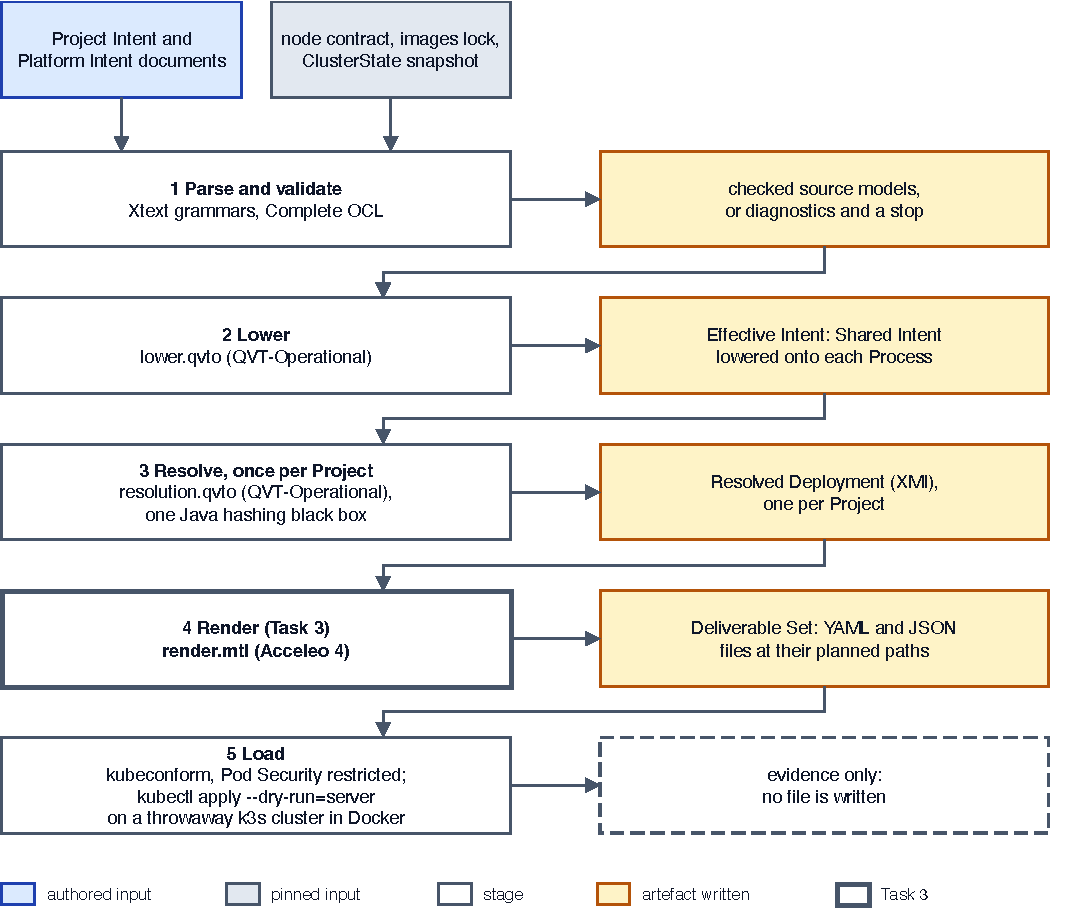
\includegraphics[width=0.82\linewidth, keepaspectratio]{Figures/pipeline}
\caption{The End-to-End Pipeline}
\label{fig:pipeline}
\end{figure}

Figure~\ref{fig:pipeline} shows five stages; Task~3 covers only rendering.
Xtext grammars and Complete OCL constraints parse and validate each document. A
QVT-Operational lowering (the flattening in Task~2) copies each Shared Intent declaration onto every
\texttt{Process} that uses it. A second QVT-Operational transformation resolves
each \texttt{Project} using the lowered models of every \texttt{Project}, the
Platform Intent and the pinned inputs. It produces one Resolved Deployment with a
path plan that assigns each Deliverable to a file. If resolution cannot derive a value,
the run stops. The Acceleo templates then run once over the set of Resolved Deployments.
Finally, the load stage checks the written files against pinned schemas, the Pod
Security \texttt{restricted} profile and a server-side dry run on a throwaway k3s
cluster (Section~\ref{sec:evaluation}).

Only resolution makes decisions; its oracle (the committed expected
models) checks them. Rendering is checked by byte comparison with the committed
\texttt{rendered} trees and by the load stage. A matching render demonstrates
correct syntax, but does not establish that the decisions were correct.

\subsection{Changes Since Task~2}
\label{sec:since-task2}

The model was refined as it was applied to production: deploying the real
estate surfaced cases the model had to express, and the changes came from those
cases. The estate pass, a third transformation over all Resolved Deployments,
was removed. The migration from the previous setup, fleet-infra with its own
DSL, was partly manual; what exists only because of it, chiefly moving data
between Instances (a Move), stems from the old deployment method rather than the
DSL, and is left out of the DSL and of this report.
Section~\ref{sec:appendix} lists each change with its reason.
% TODO(verify): confirm this summary against the appendix once it is complete.

\subsection{Roadmap}
\label{sec:roadmap}

Section~\ref{sec:alternatives} sets out the choices; Section~\ref{sec:design}
describes rendering (Figures~\ref{fig:m2t-structure} and~\ref{fig:worked-example});
Section~\ref{sec:evaluation} reports the parity and load evidence
(Figure~\ref{fig:evidence}); Section~\ref{sec:reflection} reflects on the three
tasks (Figure~\ref{fig:timeline}); Section~\ref{sec:outlook} looks beyond the
course.

% BIB: none needed in this section.

\section{Alternatives and Justification}
\label{sec:alternatives}

Table~\ref{tab:choices} summarises every decision below.

\subsection{Constraints Set by the Course}
\label{sec:fixed}

The course requires Ecore metamodels, QVT-Operational or ATL for model-to-model
transformation, Acceleo for model-to-text generation, Eclipse/EMF projects in the archive,
and a generated artefact loaded in a tool (here, the Kubernetes API server). The project
defines its own domain, target and source syntax. OCL cannot hash canonical bytes, so
one Java library computes only that digest. Maven with Tycho builds the projects
without an IDE; an examiner can also run the generator from Eclipse.

\subsection{Overview of the Design Decisions}
\label{sec:shape}

Each decision is presented with its strongest alternative and the criterion used to
reject it.

\subsubsection{Source Model: One Intent per Project, Plus a Platform Intent}
\label{sec:shape-source}

Intent is authored in one file per Project, plus one Platform Intent for facts that
must be unique across the estate
(\url{docs/adr/model/0009-intent-is-authored-one-file-per-project.md},
\url{docs/adr/model/0045-platform-intent-is-the-second-authored-document.md}). One
file per Application was rejected because each fact needs a single source: the same
OpenTelemetry variables would otherwise be repeated for three Processes. Lowering
merges shared declarations onto each Process, so templates need not combine
information from different levels.

\subsubsection{Transformation Chain: Lower, Resolve, Render}
\label{sec:shape-stages}

Three typed steps replace a single transformation from source to Resolved Deployment.
A single transformation was rejected because it obscures the source of faults: each
intermediate model has an oracle that identifies which step produced a fault.
Rendering reads only the Resolved Deployment and therefore only writes text.

\subsubsection{Removing the Estate Pass}
\label{sec:shape-estate}

The Task~2 pipeline had a third transformation over every Resolved Deployment. It
was removed because each Project owns and alone writes every object it delivers
(decision record 0116 under \path{docs/adr/model/}). Keeping it
would break the delivery guarantee that publishing an unrelated change deploys nothing: one
policy Job held every Project's grants, so one change re-ran it for all, and one
fault left seven Projects not ready. Every generated file now belongs to
one Project's Resolved Deployment, so no template merges output across Projects.

\subsubsection{Kubernetes Objects and Custom Resources as the Target}
\label{sec:shape-target}

The target consists of Kubernetes API objects and custom resources for Flux,
Flagger, the Vault Secrets Operator, Traefik and the Prometheus Operator. Flux is
the only applier, and it pulls the render by digest
(\url{docs/adr/model/0050-delivery-is-part-of-the-model.md}). A push path from CI
was rejected because it would require a deployment credential outside the cluster. Helm
or Kustomize templating was rejected because no abstract model could express its
constraints (Task~1 report). Each generated file represents an object that the API
server validates; the load stage checks this validation.

\subsubsection{One Rendering Run for All Projects}
\label{sec:shape-union}

Each Project is resolved separately using the union of all Projects, and rendering
runs once over the resulting set. Resolution from a Project's own documents alone
was rejected because it cannot account for cross-Project facts: a provider's address,
admission of a consumer by label, or rejection when a provider removes a Surface named by a consumer
(\url{spec/v1/40-composition.md}). The cost is that one Project's change can alter
another's output through names. A test checks that unrelated Projects' output remains unchanged.

\subsection{The Model-to-Text Step}
\label{sec:m2t-choices}

Rendering is the only step that writes text. Its output must match the committed
\texttt{rendered/} trees byte for byte, including whitespace, key order, quoting and headers.

\subsubsection{The Language: Acceleo 4}
\label{sec:m2t-language}

The assignment prescribes Acceleo, which also meets three technical criteria.
Acceleo~4 has a standalone API, allowing one Java class to run the module without an IDE, as in CI.
Its whitespace rules give templates exact control over the output bytes. Queries use
Acceleo Query Language (AQL) expressions over the Ecore model; the templates
are interpreted rather than compiled to Java.

The Epsilon Generation Language (EGL)~\cite{egl} also runs standalone over Ecore
and would meet the first two criteria; the assignment settles the choice. Xtend is a
separate JVM language that compiles to Java, not the template language of Xtext.
Acceleo implements the OMG standard MOFM2T~\cite{mofm2t}; no conformance is
claimed beyond the constructs the module uses.

\subsubsection{Templates Rather Than a Serialiser}
\label{sec:m2t-templates}

The production implementation uses visitors or APIs: a YAML library and a JSON encoder
write typed objects. The model-driven implementation uses templates without a subsequent
formatting pass.

The criterion is that one reviewed artefact determines the output bytes. A template
directly specifies the file layout, so a difference from the oracle points to a
visible template line. A serialiser delegates key order and quoting to library
defaults; a formatting pass adds a second tool whose version affects the bytes.
Comparing parsed documents would not check the headers, ordering or quoting
specified by the committed trees.

Two further alternatives were rejected:
\begin{itemize}
\item A model-to-model step into a Kubernetes object metamodel adds a third
metamodel of 44 object kinds that repeats the Resolved Deployment's shape, and the
target syntax still has to be written.
\item The Xtext serialiser needs a grammar and a formatter per kind, and gives no
control of the header line or key order without a custom formatter.
\end{itemize}

The cost is manual whitespace control: the template must specify every layout byte
(Section~\ref{sec:m2t-fragments}). The template also writes the key order of the
Vault JSON documents, which have no header. A string is double-quoted when a YAML implicit resolver would read it as
a null, a boolean, a number or a timestamp, or when it ends in a colon or contains
``\texttt{: }''.

\subsubsection{Template Structure: One Module with Dispatch by Type}
\label{sec:m2t-structure}

MOFM2T lets a module import others and extend or override their templates. This is
useful when a generator varies by platform. Here there is one target and no
variant to override; shared templates (label set, peer selector, consumer
label) serve nearly every kind. Splitting by kind would require imports throughout;
one module retains a single namespace. The cost is a large file navigated by template name:
3772 lines holding 113 templates and 33 queries.

YAML generation calls one overloaded \texttt{objects} template, which Acceleo resolves by the Deliverable's
runtime type (a polymorphic template in the course's terms). It replaced a chain
of 22 type tests with no \texttt{else}, where a kind without a branch produced
only the header. A kind without a template now causes the run to fail.

\subsubsection{Templates Use Only Values Present in the Model}
\label{sec:m2t-decides}

No template derives a value absent from the model. Platform decisions are made in the
QVT-Operational transformations and recorded in the Resolved Deployment, so a
missing derivation produces a missing or different file. This preserves release identity:
a release's revision is computed from the Application's canonical JSON, so a value
derived in a template would fall outside that identity.

Templates handle only target-syntax formatting. A duration becomes whole seconds,
precedence becomes a Traefik priority of 1000 minus the precedence, and a match
becomes \texttt{Path} or \texttt{PathPrefix}. The templates also apply fixed
per-kind rules of the target format: the rolling-update surge, the
\texttt{Recreate} strategy, the disruption-budget selector and the suspension of
migration Jobs. These rules do not vary by model. Queries select and order the objects
a template visits without deriving values.

\begin{table}[!htbp]
\centering
\small
\begin{tabular}{>{\raggedright\arraybackslash}p{0.15\linewidth}>{\raggedright\arraybackslash}p{0.26\linewidth}>{\raggedright\arraybackslash}p{0.25\linewidth}>{\raggedright\arraybackslash}p{0.24\linewidth}}
\hline
\textbf{Decision area} & \textbf{Rejected alternative} & \textbf{Chosen approach} & \textbf{Reason} \\
\hline
Source & One file per Application & One Intent per Project & One place per fact \\
Chain & One transformation & Lower, resolve, render & Oracle for each model \\
estate pass & Keep it & Removed & Unrelated publication deploys nothing \\
Target & Push path; Helm; Kustomize & Objects pulled by Flux & No external credential \\
Rendering input & One Project alone & Union, one run & Cross-Project facts \\
Language & EGL; Xtend & Acceleo~4 & Headless API, whitespace \\
Text output & Serialiser; formatter; parsed comparison & Templates write bytes & One artefact determines bytes \\
Other options & Model-to-model Kubernetes metamodel; Xtext serialiser & Rejected & Extra metamodel; no byte control \\
Modules & Imports, overriding & One module & No variant \\
YAML dispatch & Chain of type tests & Dispatch by type & Missing kind fails \\
Derivation & Queries in templates & Model holds values & Identity covers values \\
\hline
\end{tabular}
\caption{Summary of the Design Decisions and the Rejected Alternatives}
\label{tab:choices}
\end{table}

Section~\ref{sec:evaluation} discusses the remaining limitations and
Section~\ref{sec:reflection} the decisions that were reversed.

% BIB: \bibitem{mofm2t} Object Management Group. \emph{MOF Model to Text
%   Transformation Language (MOFM2T)}, version 1.0, 2008.
%   \url{https://www.omg.org/spec/MOFM2T/1.0/}.
% BIB: \bibitem{egl} The Epsilon Generation Language, part of the Eclipse Epsilon
%   project. \url{https://eclipse.dev/epsilon/}. TODO(verify): the authors and
%   venue from the proceedings the course material cites under Task~3.

\section{Solution Design}
\label{sec:design}

\begin{figure}[!htbp]
\centering
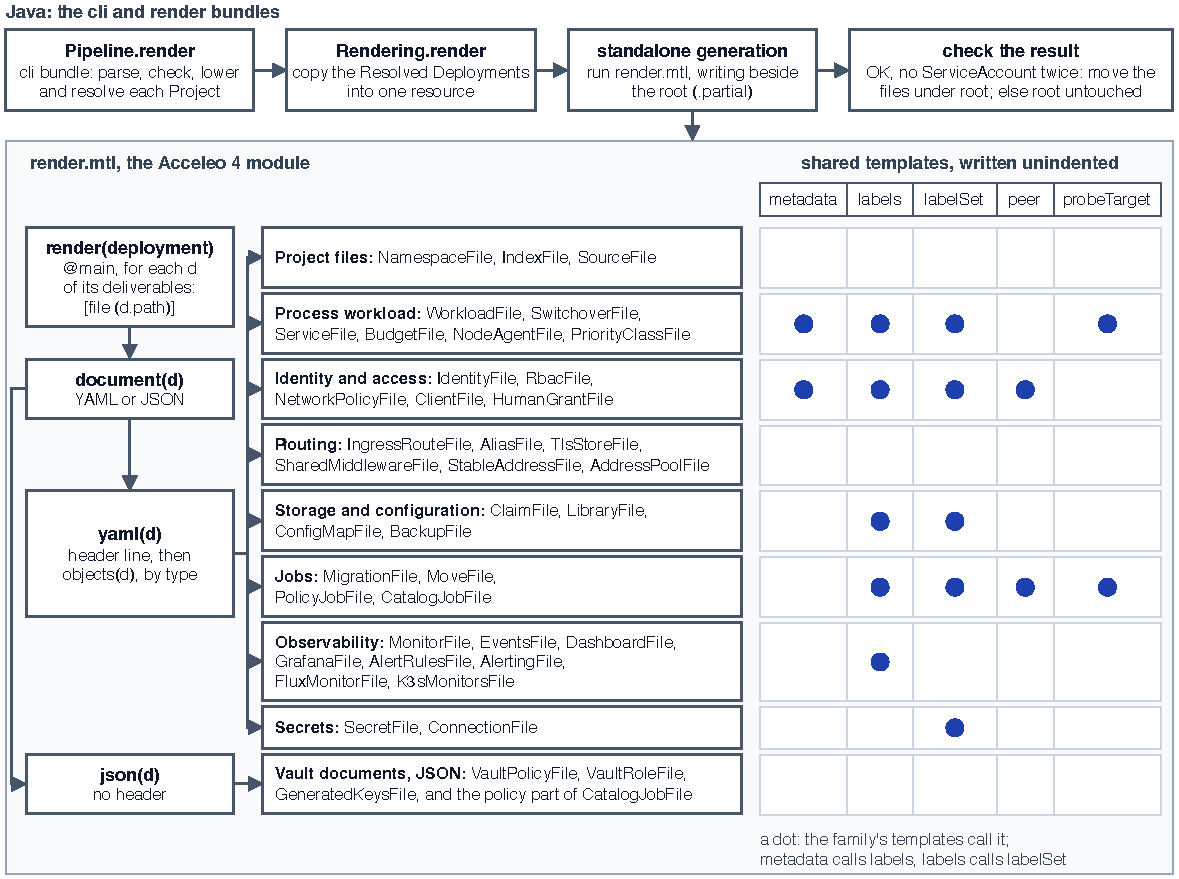
\includegraphics[width=\linewidth, keepaspectratio]{Figures/m2t-structure}
\caption{Template Structure}
\label{fig:m2t-structure}
\end{figure}
\begin{figure}[!htbp]
\centering
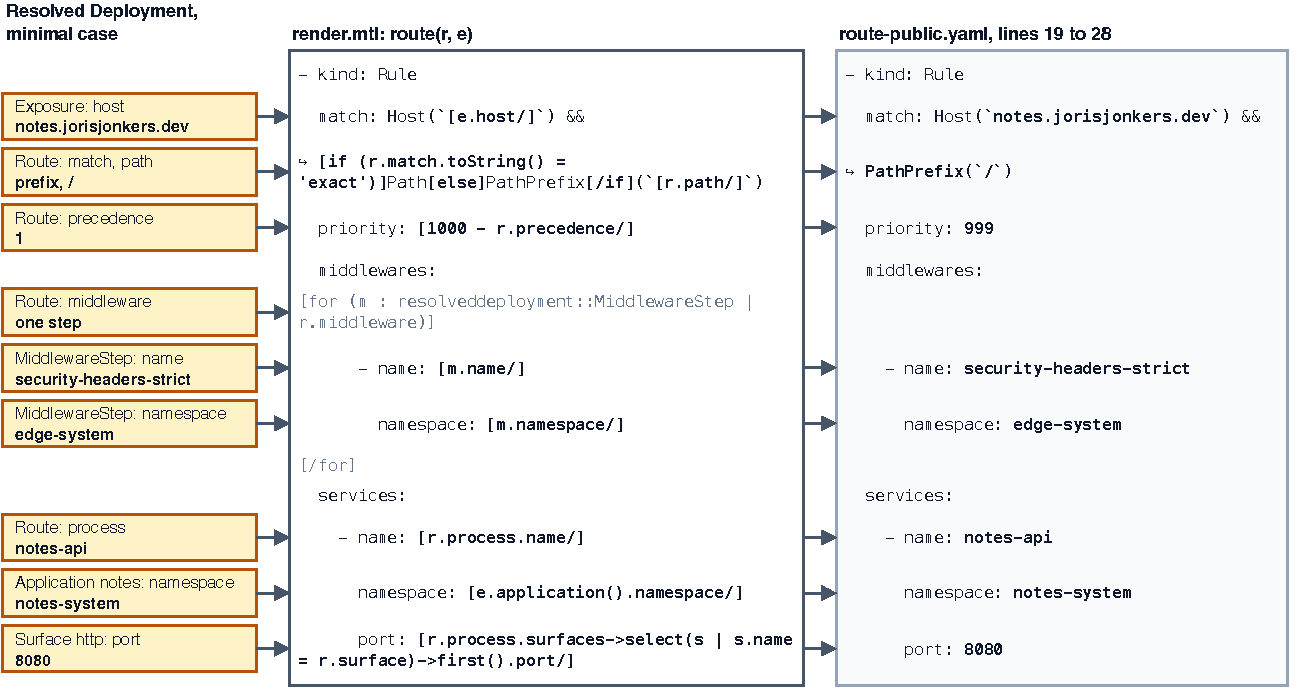
\includegraphics[width=\linewidth, keepaspectratio]{Figures/worked-example}
\caption{From Model to File}
\label{fig:worked-example}
\end{figure}

Figure~\ref{fig:m2t-structure} shows the model-to-text step: a main
template, one template family per Deliverable kind, the shared templates those
families use, and the Java class \texttt{Rendering} that loads and runs the module.
Section~\ref{sec:m2t-choices} justifies the choice of Acceleo~4. The module,
\path{emf/bundles/render/model/render.mtl}, reads the Resolved Deployment produced
by the preceding transformations. Section~\ref{sec:m2t-example} explains
Figure~\ref{fig:worked-example}, tracing one Route from model to file.

The design applies four course concepts. Dispatch by kind uses polymorphic templates
(Section~\ref{sec:m2t-kinds}). Every run regenerates every file in full, so no
protected areas are needed. Each stage is tested on its own against committed files,
and the output is held byte for byte to committed oracle files (reference trees that
both implementations must match; Section~\ref{sec:levels}), so no trace blocks map
text back to model elements. The JSON templates use text-explicit escape
(\texttt{['['/]}) to write a literal bracket.

\subsection{Interface: Input, Output and Entry Point}
\label{sec:m2t-interface}

\textbf{Input.} The step reads one Resolved Deployment for each Project in the run,
each containing a \texttt{deliverables} list of the files the Project delivers.
Lowering and resolution run for each Project in turn; \texttt{Rendering} copies the
results into one model for a single rendering run. Templates read no files,
environment variables or system clock: all other inputs are consumed beforehand
and represented as model features.
Each Deliverable has a \texttt{path} relative to the output root, assigned by the
resolution stage. The metamodel has 38 concrete Deliverable kinds
(\path{emf/bundles/metamodel/model/resolved-deployment.ecore}), each with a template
family of its own.

\textbf{Output.} The Deliverable Set contains one file per Deliverable at its
assigned path, with nothing else under the root. A YAML file begins with one header line and contains
one or more objects, each introduced by three dashes. A Vault document is JSON with no
header.

\textbf{Entry point.} The sole entry point is \texttt{Pipeline.render} in the CLI bundle. It
checks every input document. If validation rejects the set, it returns
diagnostics and writes nothing; otherwise, it lowers and resolves each Project and calls
\texttt{Rendering.render(deployments, root)} once. The step has no command-line \texttt{main}; it runs
in the Maven build of \path{emf/}, where \texttt{RenderedTreeTest} compares each
rendered file with the committed \texttt{rendered/} tree. The parity suite uses
the same entry point exclusively through files
(\path{emf/docs/adr/emf/0080-parity-crosses-the-cli-file-interface.md}).
In Eclipse, the hand-in's launch configurations run the module through the same entry point.

\subsection{The Main Template and the Path Plan}
\label{sec:m2t-main}

The seven-line main template (Example~\ref{lst:main}) opens one file per
Deliverable at the model's assigned path; it computes no paths.

\begin{lstlisting}[style=report, language=acceleo, caption={The Main Template}, label={lst:main}]
[template public render(deployment : resolveddeployment::ResolvedDeployment)]
  [for (d : resolveddeployment::Deliverable | deployment.deliverables)]
    [file (d.path, overwrite, 'UTF-8')]
      [d.document()/]
    [/file]
  [/for]
[/template]
\end{lstlisting}

The private template \texttt{document} chooses the format: JSON for the three Vault
kinds and the catalog method's policy part, YAML for everything else. YAML generation
calls \texttt{objects} on the Deliverable; Acceleo selects the overload for its
runtime type, with one overload for each of the 24 YAML kinds.

Resolution defines the path plan; templates only follow it. Each Project has
a namespace file and an index for \path{apps/<project>/}; each
Application has one file per family, with no file for a family containing no objects.
No index lists policy files or Vault documents, because the
Vault policy Job reads them from its own ConfigMap
(\path{spec/v1/30-deliverables.md}).
% TODO(verify): the claim that the ConfigMap is the only object applying the Vault
% documents is read from the path plan's description in emf/docs/architecture.md and
% spec/v1/30-deliverables.md; the full set of applying objects was not traced.

\textbf{Several Resolved Deployments, one owner per file.} A Project owns every file in
its directory, so indexes are not shared and each lists only its own Deliverable's
resources (Example~\ref{lst:index}). The composed minimal and data cases match the
two committed trees file for file (Section~\ref{sec:evaluation}).

\begin{lstlisting}[style=report, language=acceleo, caption={An Index Lists Its Own Directory}, label={lst:index}]
[template private objects(d : resolveddeployment::IndexFile)]
  ---
  apiVersion: kustomize.config.k8s.io/v1beta1
  kind: Kustomization
  resources:
  [for (r : String | d.resources->sortedBy(r | r))]
      - [r/]
  [/for]
[/template]
\end{lstlisting}

Sorting by value makes indexes independent of Deliverable order. The module
previously collected indexes through \texttt{allInstances()}; this was removed with the
estate pass (Section~\ref{sec:shape}).

Two Deliverables assigned the same path would silently overwrite the earlier file;
templates cannot detect this. The pipeline therefore checks the plan before rendering
and the written files before moving them into place, and rejects any path, ServiceAccount
or Vault name with two owners, reporting \texttt{E\_PATH\_COLLISION}
(\path{spec/v1/30-deliverables.md}).

\subsection{One Template per Deliverable Kind}
\label{sec:m2t-kinds}

The submitted module supports 38 Deliverable kinds in nine families
(Table~\ref{tab:kinds}). Each YAML family uses an \texttt{objects}
template overloaded on its receiver type. Acceleo selects the overload by runtime type
rather than string comparison: these are polymorphic templates in the course's sense.
A kind with no overload causes evaluation and the run to fail. The module previously
dispatched through 22 type tests with no \texttt{else}, so a kind without a branch
would silently produce only a header line. Type dispatch closes this gap and is 50 lines shorter.

\begin{table}[!htbp]
\centering
\small
\begin{tabular}{p{3.0cm}p{6.0cm}p{6.4cm}}
\hline
Family & Deliverable kinds & Output objects \\
\hline
Project files & \texttt{NamespaceFile}, \texttt{IndexFile}, \texttt{SourceFile} & Namespace; Kustomization; Flux \texttt{OCIRepository} and its Kustomization \\
Process workload & \texttt{WorkloadFile}, \texttt{SwitchoverFile}, \texttt{ServiceFile}, \texttt{BudgetFile}, \texttt{NodeAgentFile}, \texttt{PriorityClassFile} & Deployment (or declared controller); Flagger Canary and HorizontalPodAutoscaler; Service; PodDisruptionBudget; Node Agent DaemonSet; PriorityClass \\
Identity and access & \texttt{IdentityFile}, \texttt{RbacFile}, \texttt{NetworkPolicyFile}, \texttt{ClientFile}, \texttt{HumanGrantFile} & ServiceAccount; Role or ClusterRole and binding; NetworkPolicy; sign-in \texttt{Client}; bindings for human groups \\
Routing & \texttt{IngressRouteFile}, \texttt{AliasFile}, \texttt{SharedMiddlewareFile}, \texttt{StableAddressFile}, \texttt{AddressPoolFile} & Traefik IngressRoute with rate-limit Middleware; \texttt{ExternalName} Service; shared Middlewares; Stable Address Service; MetalLB \texttt{IPAddressPool} and \texttt{L2Advertisement} \\
Storage and configuration & \texttt{ClaimFile}, \texttt{LibraryFile}, \texttt{ConfigMapFile}, \texttt{BackupFile} & PersistentVolume and Claim; immutable ConfigMap per Asset; backup CronJob \\
Jobs & \texttt{MigrationFile}, \texttt{MoveFile}, \texttt{PolicyJobFile}, \texttt{CatalogJobFile} & Suspended Migration Jobs; Move Jobs with their Role; Vault policy and catalog Jobs by \texttt{part} \\
Observability & \texttt{MonitorFile}, \texttt{EventsFile}, \texttt{DashboardFile}, \texttt{AlertRulesFile}, \texttt{AlertingFile}, \texttt{FluxMonitorFile} & ServiceMonitor or PodMonitor; Flux Provider and Alert; \texttt{GrafanaDashboard}; \texttt{PrometheusRule}; \texttt{AlertmanagerConfig}; Flux's PodMonitor \\
Secrets & \texttt{SecretFile}, \texttt{ConnectionFile} & \texttt{VaultAuth}, \texttt{VaultStaticSecret}, \texttt{VaultDynamicSecret}; \texttt{VaultConnection} \\
Vault documents (JSON) & \texttt{VaultPolicyFile}, \texttt{VaultRoleFile}, \texttt{GeneratedKeysFile} & Policy, auth role and generated-key documents; no header \\
\hline
\end{tabular}
\caption{The 38 Deliverable Kinds in Nine Families}
\label{tab:kinds}
\end{table}

\texttt{MoveFile} renders a Move handed to it, kept for the migration (Section~\ref{sec:since-task2}).
A Deliverable represents a file rather than an object. Policy Jobs and catalog methods
are exceptions: the \texttt{part} attribute assigns each of their five objects to a
separate file, so each is planned and pruned as a separate Deliverable.

\phantomsection\label{sec:m2t-gaps}
Everything added since Task~2 followed the same sequence: a metamodel
kind or feature, its derivation in resolution, a template, and a committed file for
byte comparison. Features of existing kinds include Route annotations (facts about the
Route's tier) and the fourth Canary webhook, \texttt{rollback}, through which the
Release Gate decides whether to roll back a release it can no longer pass. Each new
kind received one \texttt{objects} overload; the edge's shared Middlewares, for
example, are named by Routes through \texttt{MiddlewareStep.name}.

Templates derive no values, but specify how the target format represents them.
The module's comments cite the chapter defining each rule:

\begin{itemize}
  \item \textbf{Update strategy.} Blue-green uses \texttt{RollingUpdate} with a surge of
    one and no unavailable pods, because Flagger starts the new version beside the old.
    Rolling uses a surge of zero and one unavailable pod, because a proxy using a host
    port cannot run two copies. Stop-start uses \texttt{Recreate}.
  \item \textbf{Disruption budget.} The selector is the resolution's \texttt{servingLabel}
    for a blue-green Process, naming the Deployment managed by Flagger
    (\texttt{serving}); otherwise, it selects the Process's own pods.
  \item \textbf{Route match.} \texttt{exact} is written as \texttt{Path}; every other match
    as \texttt{PathPrefix}.
  \item \textbf{Migration Jobs.} They are created suspended and named for their
    revision's tag. Only the Release Gate (the check that releases a migration)
    changes their suspension.
\end{itemize}
% TODO(verify): the suspended-Job rule spells the Release Gate contract of spec/v1,
% not a single model value; confirm the chapter that fixes it.

\subsection{Shared Templates and the Whitespace Rules}
\label{sec:m2t-fragments}

A shared template has multiple callers, such as the template for a Process's metadata
or label set. It is written once at the left margin; callers determine its placement.
Three whitespace rules apply. MOFM2T \S 8.4 defines what templates write at the start
and end of a line. Acceleo~4 adds two behaviours used by the module.

\textbf{The indentation margin (Acceleo~4).} Each block (the template, each \texttt{if}, each
\texttt{for}) adds two indentation spaces that Acceleo omits from the output. A line
inside $n$ enclosing blocks therefore appears $2n$ spaces further left. A Deployment's \texttt{strategy}
is indented six spaces in the module and two in the output. A negative fixture with
no body margin must fail with an Acceleo parsing error
(\path{emf/bundles/render/src/test/resources/unindented.mtl}).

\textbf{The call column (Acceleo~4).} A call repeats the text preceding it on the
line before every output line, so a shared template need not know where it will
appear. In Example~\ref{lst:labels}, \texttt{metadata} calls
\texttt{labels} at column two of its own output, and \texttt{labels} calls
\texttt{labelSet} at column zero, so the five label lines appear at column four of the
Deployment. The label set is written at the margin; its output indentation depends
on the call column.

\begin{lstlisting}[style=report, language=acceleo, caption={The Label Shared Templates}, label={lst:labels}]
[template private labels(p : resolveddeployment::ResolvedProcess)]
  [p.name.labelSet(p.component, p.application().id)/]
[/template]

[template private labelSet(name : String, component : String, application : String)]
  app.kubernetes.io/name: [name/]
  app.kubernetes.io/instance: [name/]
  app.kubernetes.io/part-of: [application/]
  app.kubernetes.io/managed-by: deploy-kit
  app.kubernetes.io/component: [component/]
[/template]
\end{lstlisting}

\textbf{List items.} A list item is a shared template that begins with its own
\texttt{- }, and the caller does not write the dash: a dash before the call would be
repeated before every line, making each line a separate item.

Whitespace is therefore a template concern (Section~\ref{sec:whitespace}). In return,
the layout is visible in the template and checked without an intervening formatter.

\subsection{Writing YAML and JSON}
\label{sec:m2t-spelling}

\textbf{Header.} A YAML Deliverable begins with \texttt{\# GENERATED. Never hand-edit.},
written once per file by \texttt{document}. A JSON document has no header, because
a comment would make it invalid for the Vault job that reads it.

\textbf{Quoting.} A string is written as a plain scalar unless the \texttt{scalar} query
matches an implicit-type pattern; matches are double-quoted. The patterns
match the whole value and cover the empty string, tilde, null, the boolean words
(\texttt{y}, \texttt{yes}, \texttt{on} and their opposites), integers in every
YAML~1.1 base, floats and timestamps.
YAML~1.1 rules are deliberate: Kubernetes tooling decodes through
\texttt{sigs.k8s.io/yaml}, which follows YAML~1.1 implicit types, and the production
implementation writes with \texttt{version: "1.1"} (\path{src/infrastructure/serializer.ts}).
A value such as \texttt{on} would reach the API server as a boolean if written as a plain scalar;
unnecessary quoting costs only bytes. The string \texttt{50} is written \texttt{"50"}.
Values a YAML reader would misread are also quoted: those opening on an indicator
character, containing \texttt{:~} or \texttt{~\#}, ending in a colon, or opening or
ending on a space. The edge's Content Security Policy, which ends in \texttt{https:},
is quoted in the committed tree.

The double-quoted form does not escape its content, so a quote or backslash in a
value would break the line. The model's value rules are intended to exclude these characters.
% TODO(verify): identify the constraint that excludes quotes and backslashes from
% scalar values.

\textbf{Block scalars.} An Asset is a file a Project ships as configuration. Its
ConfigMap holds the text as a block scalar, and its name contains a digest of the
content, so an edit produces a new immutable object
(\path{docs/adr/model/0014-file-shaped-configuration-is-an-asset.md}). Two queries
write it (Example~\ref{lst:block}).

\begin{lstlisting}[style=report, language=acceleo, caption={The Block Scalar Queries}, label={lst:block}]
[query private chomping(content : String) : String =
  if content.endsWith('\n\n') then '|+' else if content.endsWith('\n') then '|' else '|-' endif endif /]

[query private blockOf(content : String, indent : String) : String =
  (if content.endsWith('\n') then content.substring(1, content.size() - 1) else content endif)
    .replaceAll('(?m)^(?=.)', indent) /]
\end{lstlisting}

The indicator preserves trailing line breaks: one newline gives \texttt{|}
(clip), two give \texttt{|+} (keep), none give \texttt{|-} (strip). The body drops one
trailing newline, supplied by the block's own clipping, and indents every non-empty
line by four spaces; blank lines stay blank.
% TODO(verify): the substring arithmetic in blockOf uses OCL's one-based, inclusive
% substring. The committed trees agree with that reading, but the AQL reference was not
% consulted.

\textbf{Key order.} Key order follows the template text. The API reads
objects as maps, but the Acceleo~4 decision requires byte equality
(decision record 0077 under \path{emf/docs/adr/}).

\textbf{Vault documents as JSON.} A policy document has one \texttt{path}
member, with a \texttt{capabilities} list per path. A Kubernetes auth role
has three lists containing one name each. The \texttt{json} templates pretty-print
these documents with two spaces per level, using the margin rule, and escape list brackets
with \texttt{['['/]}. The policy also appears as canonical one-line JSON
in the Vault policy Job's ConfigMap, written during resolution and covered
by the digest in the ConfigMap's name. Templates do not check that the two agree;
parity comparison checks this only for committed cases.
% TODO(verify): confirm that the pretty-printed policy and the canonical document are
% generated from one value in the resolution, and not spelled separately.
A generated-key document is the only JSON file built by concatenation: the \texttt{entry}
query returns one key as an object, and \texttt{json} separates the entries with
commas. The concatenation writes keys, paths and encodings without escaping, which is
safe only while the model restricts them to characters that need none.

\subsection{Queries: Formatting and Selection}
\label{sec:m2t-queries}

The module contains 29 queries as submitted, counting each overload. Seven earlier
queries were removed because they chose values, and the
choices are now represented by model features: \texttt{allowsAt}, \texttt{policyPaths},
\texttt{catalogAllows}, \texttt{catalogPaths}, \texttt{middlewareName},
\texttt{rateLimitName} and \texttt{listed}. \texttt{serving} became \texttt{servingOf}.
Table~\ref{tab:moved-choices} lists the five choices behind them.

The remaining queries derive no model values. Formatting queries read one
value and return a string or a number (\texttt{seconds}, \texttt{octal},
\texttt{fileOf}, \texttt{directoryOf}, \texttt{writableOf}, \texttt{scalar},
\texttt{chomping}, \texttt{blockOf}, \texttt{entry}). Selection queries determine
which objects a template visits and their order (\texttt{application},
\texttt{routed}, \texttt{paths}, \texttt{hostnames}, \texttt{backups},
\texttt{backupRanges}, \texttt{files}, \texttt{destinationOf}, \texttt{versioned},
\texttt{versionOf}, \texttt{servingOf}); the module's comments specify each order.
The per-kind rules above (including \texttt{switchover} and \texttt{servingLabel})
specify how the target format represents model values without deriving them.

Each of the five choices produced a value beyond the reach of model-level tests.
These values are now derived once during resolution and only written by templates.
The trees remained identical byte for byte, except that a redirect step previously
named as a security profile by \texttt{middlewareName} is now named for its Route, as
in the production implementation.

\begin{table}[!htbp]
\centering
\small
\begin{tabular}{>{\raggedright\arraybackslash}p{0.27\linewidth}>{\raggedright\arraybackslash}p{0.33\linewidth}>{\raggedright\arraybackslash}p{0.3\linewidth}}
\hline
\textbf{Choice} & \textbf{Formerly in the template} & \textbf{Now in the model} \\
\hline
Default Vault capability & \texttt{allowsAt}: \texttt{read} for a path with no entry & \texttt{VaultPolicyFile.paths} \\
Catalog capabilities & \texttt{catalogAllows}: by the path's prefix & \texttt{ResolvedCatalogJob.policy} \\
Security profile name & \texttt{middlewareName}: by content policy & \texttt{MiddlewareStep.name}, \texttt{.namespace} \\
Rate limit name & \texttt{rateLimitName}: by the Route's position & \texttt{MiddlewareStep.name}, \texttt{.namespace} \\
Primary Deployment name & the \texttt{-primary} suffix, in two templates & \texttt{ResolvedProcess.serving}, \texttt{.servingLabel} \\
\hline
\end{tabular}
\caption{The Decisions Moved from the Templates into the Resolution}
\label{tab:moved-choices}
\end{table}

The full list of changes is in Section~\ref{sec:appendix-target} and
Section~\ref{sec:appendix-transformations}.

\subsection{The Java Class and Failure Handling}
\label{sec:m2t-java}

The Java class \texttt{Rendering} is the only Java in the step. It copies the Resolved
Deployments into a fresh resource, loads the module from the class path, and runs the
standalone generator in a \texttt{.partial} directory beside the output root. If Acceleo
reports a diagnostic other than OK, the class throws an \texttt{IllegalStateException} whose message begins
\texttt{the rendering did not complete} and includes Acceleo's text. Files move under the root
only after success, so a failed run leaves the root unchanged. A template that fails to
parse or evaluate therefore cannot silently produce an incomplete tree. The module
previously wrote directly under the root and could leave a partial tree.

\subsection{Worked Example: One Route from Model to File}
\label{sec:m2t-example}

Figure~\ref{fig:worked-example} places the model values, the Route template and the
committed YAML side by side. The minimal case has one Exposure serving
\texttt{notes.jorisjonkers.dev}, with one Route matching the path \texttt{/} as a
prefix and reaching the Process \texttt{notes-api} on its \texttt{http} Surface
(\path{spec/v1/examples/minimal/notes.project.yml}). The host and the path are
authored, and only \texttt{exact} would be written as \texttt{Path} instead of
\texttt{PathPrefix}. Resolution assigns precedence 1; the template writes
\texttt{priority: 999} by the arithmetic \texttt{1000 - r.precedence}, so that the
smallest precedence has the highest priority. The middleware step carries its name
and namespace, so the template needs no conditional choice. The module previously
chose them by the step's kind, with a query for each name (Table~\ref{tab:moved-choices}). The port
is looked up by the Surface's name among the Process's Surfaces, so the file states the
port the Process declares.

% BIB: \bibitem{yaml11} The YAML Language Development Team. \emph{YAML Ain't Markup
% Language (YAML) Version 1.1}, the type repository for the implicit types of YAML 1.1.
% \url{https://yaml.org/type/}. TODO(verify): the visit date and the exact page.
% BIB: \bibitem{acceleo4} Eclipse Foundation. \emph{Acceleo 4: Acceleo Query Language
% and the MOFM2T standalone API}. TODO(verify): the URL of the Acceleo 4 documentation
% the report should cite.
% BIB: \bibitem{ocl24} Object Management Group. \emph{Object Constraint Language},
% version 2.4, 2014. TODO(verify): the edition, for the one-based substring convention.

\section{Tests and Evaluation}
\label{sec:evaluation}

\begin{figure}[!htbp]
\centering
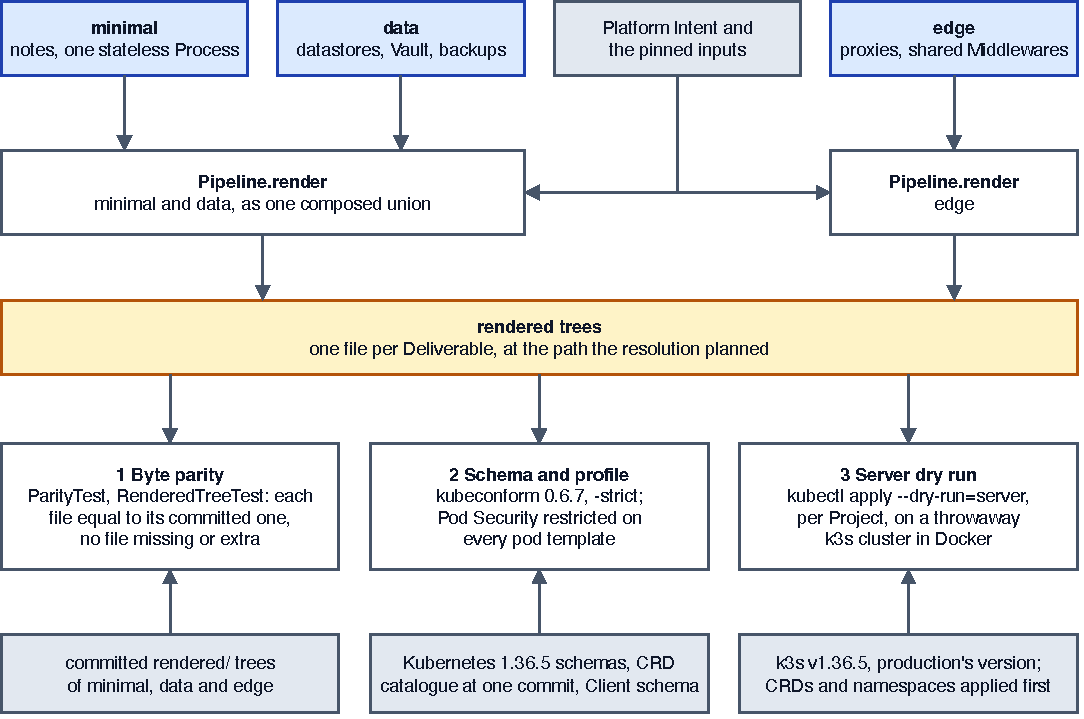
\includegraphics[width=0.92\linewidth, keepaspectratio]{Figures/evidence}
\caption{Checks from Generated Files to the Cluster}
\label{fig:evidence}
\end{figure}
% TODO(verify): Figure 4 (Figures/evidence) must show the same four levels as Table 7: template seam, CLI file interface, external schema and profile, API server.

The evaluation asks whether each transformation writes the intended model or text and whether external consumers accept the result. Committed expected files answer the first question; schema validation, a security profile and an API server address the second. Figure~\ref{fig:evidence} shows these checks along the path to the cluster.

\subsection{Testing Strategy}
\label{sec:testing-strategy}

Table~\ref{tab:checks} lists eleven checks at four levels. Each row names what the
output is compared with and the defects it can expose. Passing one check does not rule out defects covered by another.

\begin{table}[!htbp]
\centering
\small
\begin{tabular}{p{3.4cm}p{2.6cm}p{4.6cm}p{4.6cm}}
\hline
\textbf{Check} & \textbf{Level} & \textbf{Compared with} & \textbf{Defects it can expose} \\
\hline
Stage tests (\texttt{StageTest}) & 1. Stage seam & Committed expected files of each stage, each the next stage's input & A wrong value in any stage's output, named by its path \\
Field coverage (\texttt{FieldCoverageTest}) & 1. Stage seam & Every feature, literal and kind the metamodels declare & A feature no case exercises \\
Behaviour witnesses & 1. Stage seam & 75 model rows of the behaviour ledger & A model behaviour without a test \\
Seam tests (\texttt{RenderingTest}) & 1. Template seam & Expected text written in the test & A wrong header, path or key order; a template that does not parse; files left by a failed run \\
Composed union parity (\texttt{ParityTest}) & 2. CLI file interface & Committed trees of \texttt{minimal}, \texttt{data} and the platform's share & Any changed byte; a missing or extra file \\
Per-Project output (\texttt{RenderedTreeTest}) & 2. CLI file interface & Committed trees of \texttt{minimal}, \texttt{data} and \texttt{delivery} & A file written into another Project's output \\
Determinism and rejection (\texttt{RenderedTreeTest}) & 2. CLI file interface & A second run; a set the checks reject & Varying output; a partial tree on rejection \\
Oracle distance (\texttt{OracleDistanceTest}) & 2. Pipeline & Every oracle under \path{spec/v1/examples/} & An oracle on the allowlist that no longer matches \\
Schema (\path{lint:manifests}, kubeconform) & 3. External definition & Kubernetes 1.36.5 schemas, the datreeio CRD catalogue, the \texttt{Client} schema & Unknown or missing fields, wrong types \\
Pod Security (\path{scripts/lib/pod-security.ts}) & 3. External definition & Pod Security \texttt{restricted} plus a read-only root filesystem & A pod template that drops a privilege control \\
Server dry-run (k3s cluster) & 4. API server & Admission by a cluster using the production version & Objects accepted by the schema but rejected by the cluster \\
\hline
\end{tabular}
\caption{The Eleven Checks, Their Levels, Oracles and Detectable Defects}
\label{tab:checks}
\end{table}

\subsubsection{Test Levels}
\label{sec:levels}

\textbf{Stage tests.} Each transformation is unit-tested on its own: \texttt{StageTest}
runs parse, lower, resolve and render in-process, each from committed input to
committed expected files under \path{emf/bundles/cli/src/test/resources/stages/<stage>/<case>/}.
Only \texttt{parse} reads authored input; every later stage reads the expected output of
the stage before it, so one file is one stage's oracle and the next stage's input, and
two stages cannot drift apart. A render case's expected files are copies of the committed
oracles, held to them byte for byte. \texttt{FieldCoverageTest} holds each stage's cases
to every feature, enumeration literal and template dispatch its metamodels declare; the
gaps left are listed per stage in \path{gaps.txt}, a baseline that may only shrink.
Each of 75 model behaviours of the behaviour ledger has a JUnit witness
(\path{emf/docs/witnesses.md}). The build enforces 100\% line and branch coverage
(JaCoCo) and a 100\% mutation score (PIT) per module and fails below either; the
suite has 639 tests.

\textbf{Seam and file interface.} The seam tests in \path{emf/bundles/render} exercise
\texttt{Rendering} without the pipeline. A template that does not parse must fail with Acceleo's diagnostic. A template that fails halfway (\path{halfway.mtl}) must leave the output root unchanged, as the sibling \path{.partial} directory guarantees. A deliberately unindented module
(\path{unindented.mtl}) is the negative case for the indentation rule of
Section~\ref{sec:design}.
\texttt{ParityTest} in \path{emf/tests/parity} runs the whole pipeline through its
command-line file interface
(\path{emf/docs/adr/emf/0080-parity-crosses-the-cli-file-interface.md}) and checks that
the composed union contains exactly the committed files, each identical byte for byte.
\texttt{RenderedTreeTest} checks that each Project's output matches its own committed
tree, that a second run writes the same bytes, and that a set containing an invalid
document (\texttt{surface: grpc}, rejected with \texttt{E\_UNKNOWN\_SURFACE}) produces no
files. \texttt{OracleDistanceTest} measures every oracle's distance from what the
pipeline writes and holds 171 comparisons on an allowlist to an exact match.

\textbf{External consumers.} \path{scripts/lint-manifests.ts} runs kubeconform 0.6.7 with
\texttt{-kubernetes-version 1.36.5} and \texttt{-strict} against the default
schemas, the datreeio CRD catalogue and the repository's \texttt{Client} schema,
and checks every pod template against Pod Security's \texttt{restricted} profile;
both checks have negative fixtures. \path{handin/scripts/dry-run.sh}, run as
\texttt{dry-run.sh output "" generated}, applies them to the generated tree and takes about ten seconds. It then starts a disposable k3s cluster at v1.36.5, the production version, installs pinned CRDs for every non-core kind, creates the namespaces the output names and applies each Project's output and the platform's share with \texttt{-{}-dry-run=server}. An earlier attempt at 1.31 failed because the \texttt{GrafanaDashboard} CRD requires a newer API server. Network policies are absent from indexes and are applied file by file.

\subsubsection{Oracles and Their Independence}
\label{sec:oracles}

A committed file is an \emph{oracle} in this report: the expected output against
which a result is compared. The oracles under \path{spec/v1/examples/} are produced by
the production implementation; the model-driven implementation is held to them, and
its tests refuse to rewrite them. Appendix~\ref{sec:appendix-production} discusses that
implementation and the limits of this independence.

\subsubsection{Comparison: Content First, Bytes Last}
\label{sec:compare-alt}

Every intermediate model and every output is structured data, so \texttt{Comparison}
compares parsed content first and bytes last. JSON is read with Jackson, YAML with
SnakeYAML's YAML~1.1 reader on both sides, as Kubernetes reads it, so a quoted
\texttt{"on"} and a plain \texttt{on} still differ by type, and XMI is loaded into EMF
and compared with its equality helper. Every difference is reported as a path into
the document, with a list item named by its key:
\texttt{.spec.template.spec.containers[name="vault"].command: missing (expected a list of 1)}.
Only when the content agrees are the bytes compared, and a difference there is
reported as ``formatting only'', naming the first line that differs. Byte identity
remains the bar: a formatting-only difference still fails. A failure names the field
at fault instead of giving a line diff over the whole file, which made testing and
debugging faster.

\subsection{Example Models}
\label{sec:source-models}

The suite renders three examples: \texttt{minimal} (15 files, one Process with a blue-green \texttt{Canary}), \texttt{data} (76 files, five datastores and an asset-sync Process with Vault delivery) and \texttt{edge} (34 files, the two Traefik instances and a DNS controller). \texttt{minimal} and \texttt{data} render together, with the platform's four estate-scoped files,
as a composed union of 95 files, checking that adding a second Project does not
change the first Project's bytes; \texttt{edge} is compared separately.

\subsection{Results}
\label{sec:results}

Table~\ref{tab:results} reports each check for each case. The schema, profile and dry-run
results were obtained on 2026-10-31 from the generated tree. Units differ by row:
output counts refer to files; schema counts refer to resources (several may share
a file, and \path{kustomization.yaml} files count); dry-run counts
refer to objects; both include the platform's share. The profile check covers 19 pod templates; only parity reads the Vault JSON files.

\begin{table}[!htbp]
\centering
\small
\begin{tabular}{p{4.6cm}p{2.3cm}p{2.3cm}p{2.3cm}p{2.3cm}}
\hline
& \textbf{minimal} & \textbf{data} & \textbf{union} & \textbf{edge} \\
\hline
Committed files (YAML, JSON) & 15 (15, 0) & 76 (64, 12) & 95 & 34 (32, 2) \\
Written by the run & 15 & 76 & 95 & 34 \\
Byte parity & within union & within union & pass & pass \\
Per-Project output & pass & pass & -- & -- \\
Second run writes the same bytes & -- & -- & pass & -- \\
Schema (kubeconform) & 22/22 valid & 95/95 valid & -- & 44/44 valid \\
Pod Security \texttt{restricted} & no finding & no finding & -- & no finding \\
Server dry-run, indexed objects & 15/15 & 72/72 & -- & 31/31 \\
Server dry-run, network policies & 2/2 & 12/12 & -- & 5/5 \\
\hline
\end{tabular}
\caption{Results per Check and Case}
\label{tab:results}
\end{table}

The API server issued two warnings for \texttt{edge}'s public Traefik \texttt{Deployment}: two entry points are each declared twice. This reflects a modelling choice rather than a defect.

\subsection{Defects Found}
\label{sec:defects}

Most rendering defects were found by running the output rather than by byte comparison. The trees changed alongside the implementations, so comparisons passed both before and after a fix. Five examples illustrate this:
\begin{itemize}
\item A pod template omitted \texttt{allowPrivilegeEscalation: false}: found by
  reading the profile; the Pod Security check now catches it.
\item A Job's name did not reflect its pod template, so the cluster rejected it: found on a cluster; no check here catches it.
\item Eligible nodes were derived but not rendered: found by reading the adapter;
  parity catches it now.
\item A space in an authored path created a second Release Gate entry, the
  condition per Reconcile Unit that blocks a rollout: found by review; validation now rejects it.
\item An optional edge between Projects made two Reconcile Units, the units Flux
  reconciles in order, wait for each other: found in use; no example declares such an edge.
\end{itemize}

\subsection{Limitations}
\label{sec:limitations}

\paragraph{Template coverage.} Comparisons provide no evidence about kinds absent from the compared trees; the render stage's baseline names each one.
Acceleo template coverage is not measured: the gates do not reach templates, and no
tool reports which branches the cases exercise. A one-character change to the Namespace
template's \texttt{managed-by} label failed 14 of 25 stage cases and 5 of 9 rendered-tree
tests, each naming the file; a change to a kind no compared tree holds would pass.

\paragraph{Version pins.} Schema validation is pinned to Kubernetes 1.36.5 and one
CRD catalogue commit, while production worker nodes run 1.35.2. A field ignored by a
1.35 kubelet would therefore pass validation.

\paragraph{Fresh-cluster dry-run.} This cannot detect defects involving immutable fields; no controllers run and no network policies are enforced. The
model-driven implementation does not apply objects, so these checks do not exercise
Flux's ordering, pruning or release gating.

\paragraph{When the build runs.} The \texttt{Model-driven build} job runs the Maven
verify, tests and the coverage gate, on every commit that changes \path{emf/} or the
workflow; other changes skip it. The mutation gate takes too long for every change and runs
nightly instead. A Maven
wrapper update once broke the Tycho build unnoticed while it ran only on request: an
implementation stays level with shared oracles only while every change that reaches it
runs its build.

\section{Reflection}
\label{sec:reflection}

The project ran from the Task 0 proposal in September to this submission on
30 October. Figure~\ref{fig:timeline} places the three tasks, both presentations
and the project's phases on one timeline, beside the commits per day.

\begin{figure}[!htbp]
\centering
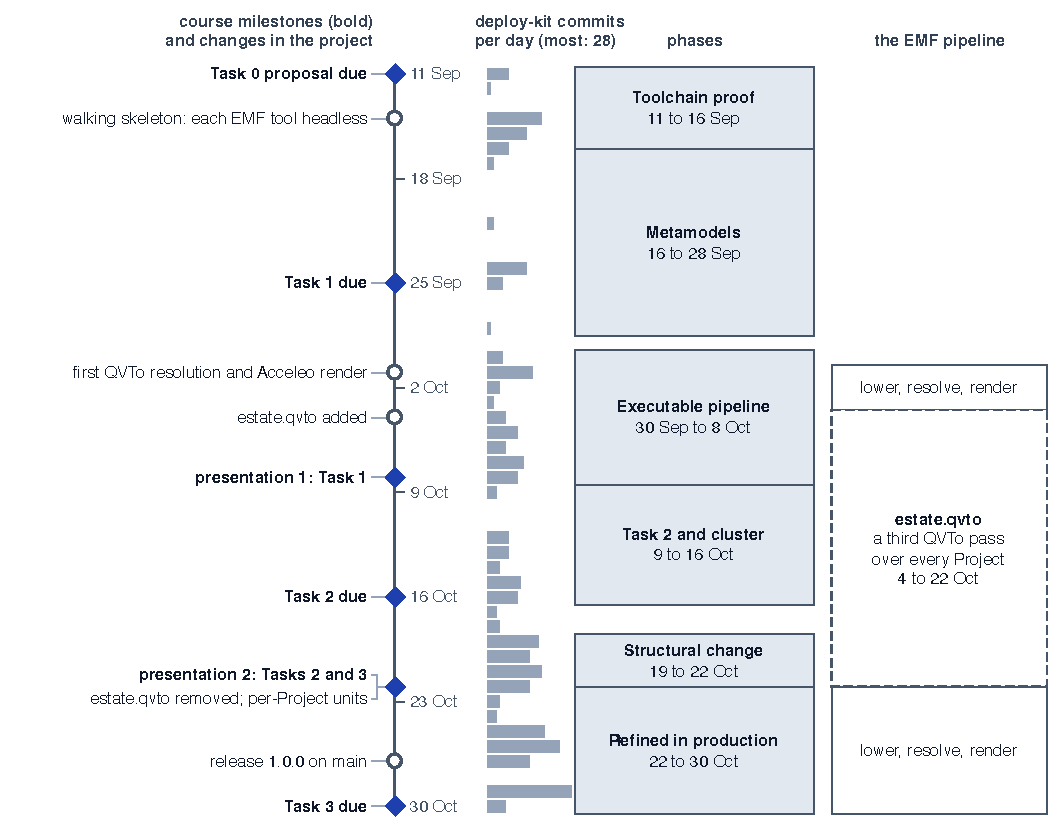
\includegraphics[width=0.78\linewidth, keepaspectratio]{Figures/timeline}
\caption{Project Timeline}
\label{fig:timeline}
\end{figure}
% TODO(verify): Figure 5 (Figures/timeline) must start phase 1 on 14 September (first commit under emf/) and show the Task 1 presentation on 8 October.

\subsection{How the Project Changed Over Time}
\label{sec:timeline-narrative}

The proposal fixed a closed set of inputs, an intermediate Resolved Deployment, a
generated Deliverable Set and two implementations tested against the same examples,
but left the build order open. Priorities shifted through six phases.
\begin{itemize}
\item 14 to 16 September: demonstrating that each tool could run, through the
  headless build, the oracle layout and the parity seam.
\item 16 to 28 September: the metamodels, ending in the Task 1 submission on
  25 September.
\item 30 September to 8 October: the pipeline became executable, with the first
  byte-for-byte Acceleo rendering of \texttt{minimal} on 1 October.
\item 9 to 16 October: the Task 2 report, written after the Task 1 presentation
  on 8 October.
\item 19 to 22 October: the estate pass was removed (Section~\ref{sec:shape-estate});
  the second presentation was on 22 October.
\item 22 to 30 October: the model was refined in production and reached release
  1.0.0; the model-driven implementation adopted each change. In October, the
  repository received 275 commits, 168 of which touched \path{spec/v1}.
\end{itemize}
Three factors drove these shifts: deadlines three weeks apart and then two, cases
surfaced in production, and oracle changes the model-driven implementation had to
follow.

\subsection{What Went Well}
\label{sec:went-well}

\subsubsection{Oracle Parity Across Two Implementations}
\label{sec:went-parity}

Both implementations are held to the same committed oracles, and neither is
generated from the other, so they converged on the same behaviour
(Appendix~\ref{sec:appendix-production}). Section~\ref{sec:oracles} explains the limits of this
evidence.

\subsubsection{Specification and Decisions Before the Reports}
\label{sec:went-spec}

The normative model and the decision records were written before the reports, so
a report could cite the record justifying each decision. The rendered tree of
\texttt{minimal} was committed on 8 September, three weeks before the first
Acceleo template, so it specified the expected output independently of the templates.

\subsubsection{A Headless EMF Toolchain}
\label{sec:went-headless}

Maven with Tycho runs every EMF tool without an IDE, using one dated Eclipse release.
A walking skeleton, metamodel, OCL file and template each ran through its own tool
before substantive content was added. When the Acceleo module arrived on
1 October, subsequent failures therefore concerned content.
% TODO(verify): "every stage run" assumes the CI job runs the full pipeline under mvn verify; confirm against emf/pom.xml.

\subsubsection{Output Tested Against a Live Cluster}
\label{sec:went-cluster}

Applying generated files to a real cluster exposed faults beyond parsers and unit
tests: an immutable Deployment selector, Jobs requiring recreation, and an omitted
Pod Security control. This motivated the server dry-run in Section~\ref{sec:levels}.
% TODO(verify): each cluster fault was found on the cluster rather than in review; the commit subjects support the claim but not the mechanism.

\subsection{What Could Have Been Better}
\label{sec:could-better}

\subsubsection{Structural Changes After Task 2}
\label{sec:late-structure}

The Task 2 report describes three transformations; the estate pass was removed
four days after it was rewritten, so the report is a snapshot of a pipeline that
no longer exists. The appendix records the difference, but the structure should
have been fixed at the Task 2 deadline, with later structural decisions recorded
as changes.

\subsubsection{Acceleo's Whitespace Rules}
\label{sec:whitespace}

Byte comparison directed much of the template work towards presentation. Acceleo 4 strips
a margin from each block-body line; a call repeats the text preceding it on the
line before every output line, so shared templates are written without
indentation (Section~\ref{sec:design}). The \texttt{GENERATED} header, key order
and quoting rule were template decisions made to match the oracle. The effort
concerned output appearance, not transformation semantics.

\subsubsection{Scope}
\label{sec:scope}

The scope was too large for one course. Between 14 September and 30 October, the
repository received 341 commits across the specification, the production
implementation and \path{emf/}, a second implementation of the whole compiler,
and keeping the two level doubled every change. A smaller scope would
have kept the parity, decision records and headless build, held the model at its
Task 1 scope and documented later features as deferred.

\subsubsection{Structural Comparison Came Late}
\label{sec:byte-cost}

For most of the project, output was compared only as bytes: a line diff across
several hundred lines does not distinguish missing keys, extra keys and wrong values.
The structured comparison of Section~\ref{sec:compare-alt} names each difference's
path; adopting it from the start would have saved much debugging.

\subsection{What Was Learned}
\label{sec:learned}

\subsubsection{Decide in the Transformation, Write in the Template}
\label{sec:decide-spell}

Model-to-model transformations make decisions; templates write the results.
When templates derive no values absent from the model, output errors can be traced
either to the model or to target-syntax formatting. The model can then be tested
independently of the template.

\subsubsection{Metamodels as Contracts Between Stages}
\label{sec:contracts}

Typing each stage's model catches errors earlier and makes each stage
replaceable: the estate pass was removed without changing the parser or the
renderer. The cost is that each metamodel changes when its stage does.

\subsubsection{The Cost of Running MDE Tools Without an IDE}
\label{sec:headless-cost}

Most of the effort in model-driven tooling went into running it rather than modelling.
The module's POM changed in at least ten commits, and the indentation rule was established
experimentally. Build configuration and documented tool behaviour therefore deserve
at least as much attention as metamodels.

\subsubsection{Compare Parsed Documents Before Bytes}
\label{sec:structural-oracles}

Oracles should be compared as parsed documents first, then as bytes, and each
stage tested on its own: a failure then names the stage and the field at fault
(Section~\ref{sec:compare-alt}).

% TODO(verify): the Task 0 approval date is recorded only as "September"; confirm the exact date from the course's Canvas record before the hand-in.

\section{Outlook}
\label{sec:outlook}

The project continues in a new repository with one Rust codebase for the
compiler and in-cluster service. The web interface remains in Vue and uses
the Rust API. The oracle files and parity method carry over: the Rust
compiler must match the committed files under \path{spec/v1/examples/}, and a
difference between implementations remains a defect in one of them. The
model-driven implementation (\path{emf/}) will be retired after the grade is recorded;
it served as the model-driven reference against which the oracles were first checked.




\begin{thebibliography}{9}
\bibitem{mofm2t} Object Management Group. \emph{MOF Model to Text
  Transformation Language (MOFM2T)}, version 1.0, 2008.
  \url{https://www.omg.org/spec/MOFM2T/1.0/}.
\bibitem{egl} L.~M.~Rose, R.~F.~Paige, D.~S.~Kolovos and F.~A.~C.~Polack.
  The Epsilon Generation Language. In \emph{Model Driven Architecture --
  Foundations and Applications (ECMDA-FA 2008)}, LNCS 5095, Springer, 2008.
\end{thebibliography}

%==== APPENDIX ====
\clearpage
\appendix
\section{Changes to the Task 1 Metamodels and Task 2 Transformations}
\label{sec:appendix}

This appendix lists changes to the Task~1 metamodels and Task~2 transformations
in the Task~3 pipeline, organised by artefact. The baseline is the Task~2
submission's metamodel appendix and design section. These describe three
QVT-Operational transformations (lowering, resolution and the estate pass
over the Resolved Deployments) and the Task~1-to-Task~2 metamodel changes.
Each subsection contains tables with one row per change, identifying the
affected classes and features and briefly explaining the reason.

The model was refined as it was applied to production: deploying the real
estate surfaced cases the model had to express, and the changes below came from
those cases. The tables group them by theme; changes that concern only the
model-driven implementation, not the model, form a group of their own. The
change set was derived from the repository's git history rather than a
comparison of complete models, so each row summarises a commit's effect.

File sizes indicate the extent of the changes. As submitted, the Project Intent
metamodel, which also holds the Platform Intent classes, has 137 classes and
441 features, the Resolved Deployment metamodel 133 classes and 619 features,
and the Pinned Inputs metamodel 15 classes and 67 features. The resolution
transformation has 4276 lines, 10 mappings and 305 queries, and the lowering
has 473 lines and 54 mappings, compared with about 1700 and 340 lines in the
Task~2 design section. The 134-line estate pass was removed. The Acceleo
module has 3772 lines.

\subsection{Source Metamodel (Project Intent)}
\label{sec:appendix-source}

The source metamodel defines what an author writes in a Project's files.
Figure~\ref{fig:mm-source} shows its Project Intent part. Changes fall into five
themes: how a \texttt{Process} reaches platform services, how it receives secrets,
the identity and placement constraints checked by the model, further forms of
\texttt{Process}, and the exposure, sign-in and observation of an
\texttt{Application}. The Platform Intent classes live in
the same \path{project-intent.ecore} file, and Section~\ref{sec:appendix-platform}
covers them separately.

\begin{figure}[!htbp]
\centering
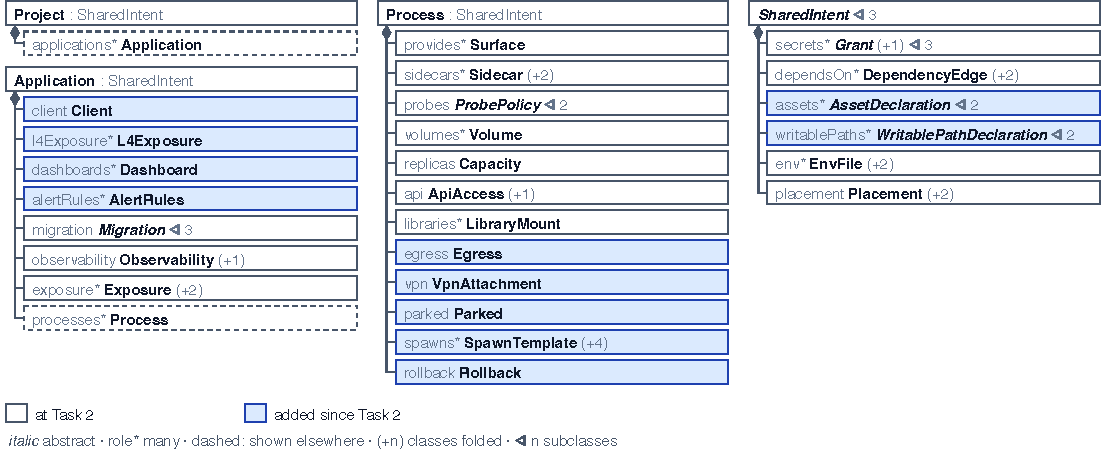
\includegraphics[width=\linewidth, keepaspectratio]{Figures/mm-source}
\caption{The Source Metamodel as Submitted}
\label{fig:mm-source}
\end{figure}

These changes keep authored documents small. Each new field records a choice
the author must make or a reason the model could not infer. No field is added
where a platform fact already determines its value.

\begin{table}[!htbp]
\centering
\footnotesize
\begin{tabular}{>{\raggedright\arraybackslash}p{\dimexpr0.22\linewidth-2\tabcolsep}>{\raggedright\arraybackslash}p{\dimexpr0.48\linewidth-2\tabcolsep}>{\raggedright\arraybackslash}p{\dimexpr0.30\linewidth-2\tabcolsep}}
\hline
\textbf{Change} & \textbf{What changed} & \textbf{Why} \\
\hline
\multicolumn{3}{l}{\textit{Reaching the platform's services}} \\
Process VPN attachment & \texttt{Process} gains \texttt{vpn}, a \texttt{VpnAttachment} holding one \texttt{forwardedPort}. Its image, credential and resource quantities come from Platform Intent. & The author specifies only the forwarded port, without tunnel details. \\
Internet egress & \texttt{Process} gains \texttt{egress}, containing \texttt{to} entries of \texttt{EgressTarget} and a required \texttt{reason}. & Default deny remains the rule; each exception has a declared reason for review. \\
Library mount & \texttt{Process} gains \texttt{libraries}: \texttt{LibraryMount} (\texttt{library}, \texttt{mountAt}, \texttt{subPath}) with a \texttt{LibraryAccess}. & A library is a directory on one node. The mount names it and requests access, which is checked against the grant. \\
GPU placement & Placement gains a structured \texttt{gpu} with a vendor and model. & One declaration selects and requests a card, so the request is derived without repetition. \\
\multicolumn{3}{l}{\textit{Secrets and keys}} \\
Declared secret keys & The flat key list becomes \texttt{KvKey}, a \texttt{name} with either \texttt{PlainKey} or \texttt{GeneratedKey}. \texttt{GeneratedKey} holds \texttt{generate}: \texttt{bytes} and an \texttt{encoding} of \texttt{KeyEncoding}. & A platform-generated key is declared by its shape; its value never enters the model. \\
Credential delivery & A grant's delivery target gains \texttt{mountAt} and \texttt{fileMode}, allowing an edge's credential to be delivered as a file with its own mode, alongside environment delivery. & A Process may require file delivery; the file's location and mode form part of the contract. \\
Transit read & A transit grant may declare \texttt{read}, covering the key's public part. & A JWKS endpoint needs only the public part. \\
\multicolumn{3}{l}{\textit{Identity and constraints}} \\
Consumer addresses by Application Id & An edge names its provider by Application Id, checked by the \texttt{DependencyEdges} descriptor and an OCL constraint. & Consumer configuration depends only on the Id, never on a namespace or Project. \\
Unique claim reservation & An OCL constraint rejects a \texttt{claim} reserved by two volumes in one Project. & A Project's Processes share a namespace, so two volumes using one claim would silently share data. \\
\hline
\end{tabular}
\caption{Changes to the Project Intent Metamodel Since Task~2: Reaching the Platform's Services; Secrets and Keys; Identity and Constraints}
\label{tab:app-source}
\end{table}

\begin{table}[!htbp]
\centering
\footnotesize
\begin{tabular}{>{\raggedright\arraybackslash}p{\dimexpr0.22\linewidth-2\tabcolsep}>{\raggedright\arraybackslash}p{\dimexpr0.48\linewidth-2\tabcolsep}>{\raggedright\arraybackslash}p{\dimexpr0.30\linewidth-2\tabcolsep}}
\hline
\textbf{Change} & \textbf{What changed} & \textbf{Why} \\
\hline
Command and memory-backed paths & A Process and a sidecar may declare \texttt{command} and \texttt{args}, lists of literal words replacing the image's entrypoint and arguments; a writable path may be \texttt{\{path, memory\}}. & Image startup concerns only its Process, so words cannot contain placeholders; memory-backed paths count towards that Process's memory. \\
API access scope & \texttt{ApiRule} is scoped to the Process's namespace or the cluster. A Process can access the Kubernetes API without a rule when its declaration suffices. & Access is declared at the required scope and no wider. \\
Spawn templates & A Process may create pods only from a declared spawn template. & Dynamic workloads are restricted to declared shapes. \\
Sidecar volumes and init & A \texttt{Sidecar} mounts the named Process volumes and may run before the main container as an init step. & A sidecar needs access to its data, with execution order declared. \\
Lifecycle: scheduled and parked & \texttt{lifecycle} may be \texttt{scheduled} with its own cron schedule; a Process may be \texttt{parked} with a \texttt{reason}. & A scheduled Process renders a CronJob; a parked Process retains its claims and grants without running pods. \\
Capacity across nodes & A \texttt{Capacity} exception may specify \texttt{across: node}. & Replicas spread across nodes without a second rule. \\
Low port & A Process may listen below 1024. & The substrate binds any port without a capability, preserving the restricted posture. \\
\hline
\end{tabular}
\caption{Changes to the Project Intent Metamodel Since Task~2: Process Forms and Their Constraints}
\label{tab:app-source-2}
\end{table}

\begin{table}[!htbp]
\centering
\footnotesize
\begin{tabular}{>{\raggedright\arraybackslash}p{\dimexpr0.22\linewidth-2\tabcolsep}>{\raggedright\arraybackslash}p{\dimexpr0.48\linewidth-2\tabcolsep}>{\raggedright\arraybackslash}p{\dimexpr0.30\linewidth-2\tabcolsep}}
\hline
\textbf{Change} & \textbf{What changed} & \textbf{Why} \\
\hline
Raw Surfaces & An \texttt{Application} gains an \texttt{l4Exposure} (port, protocol, address, Process, Surface); a Surface may use a node's own address. & Raw TCP and UDP services receive a declared address. \\
Route rate limit & A Route gains \texttt{RateLimit} with \texttt{requests} and \texttt{per}. & A Route may limit requests per client; the proxy enforces this limit. \\
Route redirect & A Route gains \texttt{redirectTo}, rendered as a separate Middleware. & A redirect belongs to its Route. \\
Client block & An \texttt{Application} gains a \texttt{client} block with the sign-in fields required by its mode. & Sign-in is declared by the Application using it. \\
Dashboards and alert rules & The \texttt{Application} declares its Grafana dashboards and alert rules. & Observation is declared alongside the observed Application. \\
\hline
\end{tabular}
\caption{Changes to the Project Intent Metamodel Since Task~2: Exposure, Sign-in and Observability}
\label{tab:app-source-3}
\end{table}

The OCL constraints also changed substantially. The constraints above are among
them, and each new form of \texttt{Process} brought its own constraints into
\path{project-intent.ocl}.

\subsection{Platform Intent}
\label{sec:appendix-platform}

The platform team writes one Platform Intent for the estate. It defines choices
unavailable to Projects: privileged roles, engines and their catalog methods,
images for platform components, resources available to Processes and
the policies limiting their use. Figure~\ref{fig:mm-platform} shows its classes.
Its metamodel is the Platform part of \path{project-intent.ecore}; its grammar is
\path{PlatformIntent.xtext}.

\begin{figure}[!htbp]
\centering
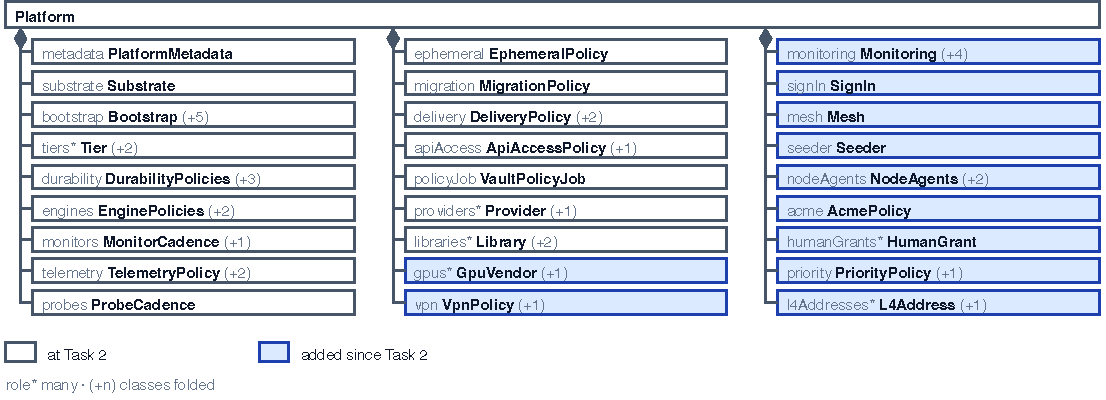
\includegraphics[width=\linewidth, keepaspectratio]{Figures/mm-platform}
\caption{The Platform Intent Metamodel as Submitted}
\label{fig:mm-platform}
\end{figure}

Platform Intent changed in two ways. First, the eight privileged-role fields
now name both a Project and an Application, breaking compatibility with every
document that sets them. Second, it gained policies previously held in
transformations or Project files: the VPN image, GPU resource names, library
grants and each engine's catalog method.

\begin{table}[!htbp]
\centering
\footnotesize
\begin{tabular}{>{\raggedright\arraybackslash}p{\dimexpr0.22\linewidth-2\tabcolsep}>{\raggedright\arraybackslash}p{\dimexpr0.48\linewidth-2\tabcolsep}>{\raggedright\arraybackslash}p{\dimexpr0.30\linewidth-2\tabcolsep}}
\hline
\textbf{Change} & \textbf{What changed} & \textbf{Why} \\
\hline
\multicolumn{3}{l}{\textit{Privileged roles and human access}} \\
Roles name their Project & The eight fields giving an \texttt{Application} a privileged role take \texttt{<project>/<application>}, resolved in \path{ProjectIntentScopes.java}. This breaks compatibility with every Platform Intent. & An Application Id can be declared in any Project's file; a bare Id cannot identify its Project. \\
Human grants & \texttt{humanGrants}: each entry contains a \texttt{group} (as seen by the API server), one of four built-in cluster roles, and a \texttt{reason}. & The platform decides who administers the cluster, so grants belong to no Application. \\
\multicolumn{3}{l}{\textit{Engines}} \\
Catalog method & An engine entry names a \texttt{catalog} method: an image that applies a catalog through the engine's Surface, with its user and sign-in. & Applying a database catalog writes to a live datastore using a privileged identity. The platform specifies each engine's method; the transformation only plans the Job. \\
New engines & \texttt{mongo} joins the engine vocabulary, and \texttt{s3} gains a bucket catalog method. & No catalog is derived for a store without databases; object-store keys and buckets are derived from edges. \\
\multicolumn{3}{l}{\textit{Resources available to Processes}} \\
VPN policy & \texttt{VpnPolicy}: an image, a credential, \texttt{memory} and \texttt{cpu}, and \texttt{VpnSetting} key-value entries. & The tunnel's image and settings are platform facts that no Project should set. \\
GPU vendors & \texttt{GpuVendor} with \texttt{GpuVendorPolicy}: a \texttt{resource} name and a \texttt{runtimeClass}. & The resource name and runtime class belong to the driver the platform runs. \\
Libraries & \texttt{LibraryDeclaration} with \texttt{Library} entries: a directory on one node and the Projects granted access. & The platform names directories and grants access; Projects mount only those granted to them. \\
Substrate pulls & The substrate's image pull is allowed within every derived deadline. & A deadline derived for another purpose must not cause an image pull to fail. \\
\hline
\end{tabular}
\caption{Changes to the Platform Intent Since Task~2: Privileged Roles and Human Access; Engines; Resources Available to Processes}
\label{tab:app-platform}
\end{table}

\begin{table}[!htbp]
\centering
\footnotesize
\begin{tabular}{>{\raggedright\arraybackslash}p{\dimexpr0.22\linewidth-2\tabcolsep}>{\raggedright\arraybackslash}p{\dimexpr0.48\linewidth-2\tabcolsep}>{\raggedright\arraybackslash}p{\dimexpr0.30\linewidth-2\tabcolsep}}
\hline
\textbf{Change} & \textbf{What changed} & \textbf{Why} \\
\hline
Tier forward auth & A tier's \texttt{forwardAuth} names a provider Application, its responding Surface and the path. & The endpoint follows the provider's Process, so moving the provider updates the edge's target. \\
Tier certificates and addresses & A tier gains an L4 Address and its own certificate; a Route takes its TLS from its tier. & Each tier is a proxy with its own entry point and certificate. \\
Tier DNS and ingress class & A tier declares \texttt{dns} (\texttt{target}, \texttt{proxied}) and an ingress class. & Routes carry the annotations required by public records and the selected proxy. \\
Default certificate & A tier that issues no certificate names a Secret Store path in \texttt{certificateFrom}. & Every proxy serves that certificate to a Route naming none of its own. \\
L4 Addresses & Named L4 Addresses, each an IPv4 pool announced at one site. & A raw Surface needs a platform-owned address. \\
Mesh enrolment & \texttt{mesh.enrolled} names the Projects in the ambient mesh. & Enrolment is the platform's decision, and a name no Project declares is rejected. \\
\hline
\end{tabular}
\caption{Changes to the Platform Intent Since Task~2: Tiers, the Edge and the Mesh}
\label{tab:app-platform-2}
\end{table}

\begin{table}[!htbp]
\centering
\footnotesize
\begin{tabular}{>{\raggedright\arraybackslash}p{\dimexpr0.22\linewidth-2\tabcolsep}>{\raggedright\arraybackslash}p{\dimexpr0.48\linewidth-2\tabcolsep}>{\raggedright\arraybackslash}p{\dimexpr0.30\linewidth-2\tabcolsep}}
\hline
\textbf{Change} & \textbf{What changed} & \textbf{Why} \\
\hline
Flux metrics & The bootstrap set's Flux entry records the port and path where its controllers serve metrics. & Flux serves all Projects and belongs to none, so the platform records how to reach it. \\
k3s metrics and monitoring stores & The bootstrap set's \texttt{k3s} entry (\texttt{K3sInstall}, \texttt{K3sMetrics}) records where the kubelet, the API server and the cluster DNS serve metrics; \texttt{Monitoring} gains \texttt{stores}, the Loki, Tempo and Pyroscope Applications Grafana reads. & The cluster's own components and Grafana's data sources belong to no Project, so the platform records them. \\
Priority classes & Two classes, \texttt{data} and \texttt{critical}, and a list of critical Applications. & Priority is derived from the Process rather than authored by it. \\
Node agents & Node agents are derived from node facts and pools. & Agents follow existing nodes without a duplicated list. \\
Foundation and bootstrap set & The remaining foundation and its bootstrap set are declared. & The platform specifies what a cluster needs before any Project runs. \\
Off-cluster recipient & Each off-cluster copy is encrypted to a platform-named recipient. & Only the holder of the recipient's key may read the copy. \\
DNS resolution & A DNS-serving Process resolves through the platform's upstream nameservers. & The resolver's upstream is a platform fact. \\
\hline
\end{tabular}
\caption{Changes to the Platform Intent Since Task~2: Scheduling, Priority and the Foundation}
\label{tab:app-platform-3}
\end{table}

\subsection{Pinned Inputs}
\label{sec:appendix-pinned}

Pinned inputs are documents read during resolution but not written by an author:
the images lock, node contract and ClusterState snapshot. Their classes are
defined in \path{pinned-inputs.ecore} and shown in Figure~\ref{fig:mm-pinned}.
The changes concern the images lock's versions and checks, and the snapshot's
backup list.

\begin{figure}[!htbp]
\centering
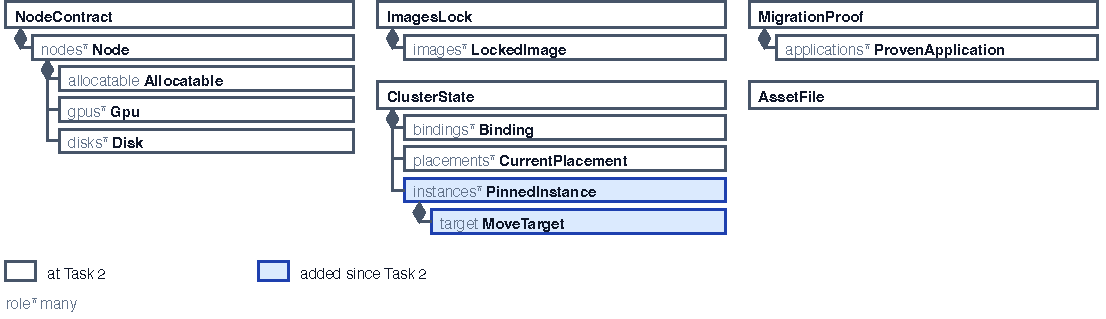
\includegraphics[width=\linewidth, keepaspectratio]{Figures/mm-pinned}
\caption{The Pinned Inputs Metamodel as Submitted}
\label{fig:mm-pinned}
\end{figure}

\begin{table}[!htbp]
\centering
\footnotesize
\begin{tabular}{>{\raggedright\arraybackslash}p{\dimexpr0.22\linewidth-2\tabcolsep}>{\raggedright\arraybackslash}p{\dimexpr0.48\linewidth-2\tabcolsep}>{\raggedright\arraybackslash}p{\dimexpr0.30\linewidth-2\tabcolsep}}
\hline
\textbf{Change} & \textbf{What changed} & \textbf{Why} \\
\hline
\multicolumn{3}{l}{\textit{Images lock}} \\
Version on every entry & Each images-lock entry gains \texttt{version}, a \texttt{String} in \path{pinned-inputs.ecore} and \path{ImagesLock.xtext}. Rendering writes it on every pod running the image. & A pod must identify its software release. \\
Rejection of missing versions & The grammar accepts an entry without \texttt{version}; resolution rejects it as \texttt{E\_IMAGE\_VERSION\_MISSING}. & This identifies the model entry, whereas a grammar error would identify only the line. \\
Root rejected & An image locked with uid 0 is rejected as \texttt{E\_IMAGE\_RUNS\_AS\_ROOT}. & The hardening posture requires a non-root uid, which a root image cannot supply. \\
\multicolumn{3}{l}{\textit{ClusterState snapshot}} \\
Backups removed & The snapshot's rollback-backup list and annotation are removed. & Rollback uses scheduled backups, so the snapshot no longer records an unused backup. \\
\hline
\end{tabular}
\caption{Changes to the Pinned Inputs Since Task~2: Images Lock; ClusterState Snapshot}
\label{tab:app-pinned}
\label{tab:app-pinned-2}
\end{table}

Output remains a function of the pinned inputs. A fact about the running cluster
therefore enters as a new pinned value, rather than a live-cluster read. Section~\ref{sec:design} covers the snapshot rules and the reason the node
contract records capacity; they are not repeated here.

\subsection{Target Metamodel (Resolved Deployment)}
\label{sec:appendix-target}

Resolution produces the Resolved Deployment; rendering reads it. It grew in two
areas: values derived per Project and features required by workloads.
Figure~\ref{fig:mm-target} shows the metamodel. As in Task~2, there is one root
instance per Project, but its values now belong to that Project. In Task~2,
every Project recorded the same Vault policy Job and rollout events. Each now
has its own values, delivered by its own Reconcile Unit.

\begin{figure}[!htbp]
\centering
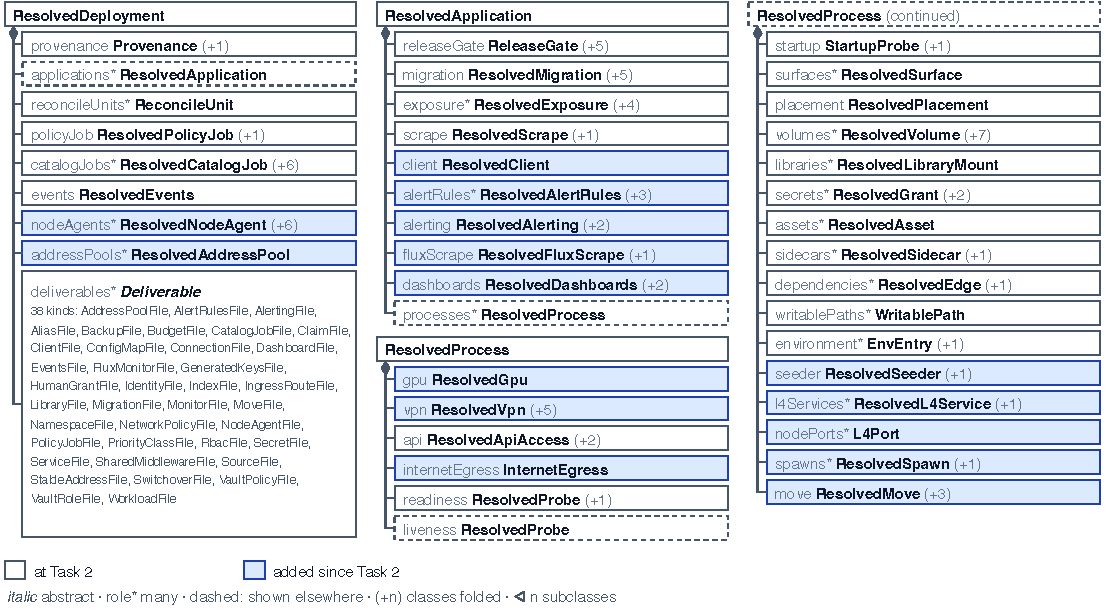
\includegraphics[width=\linewidth, keepaspectratio]{Figures/mm-target}
\caption{The Target Metamodel as Submitted}
\label{fig:mm-target}
\end{figure}

\begin{table}[!htbp]
\centering
\footnotesize
\begin{tabular}{>{\raggedright\arraybackslash}p{\dimexpr0.22\linewidth-2\tabcolsep}>{\raggedright\arraybackslash}p{\dimexpr0.48\linewidth-2\tabcolsep}>{\raggedright\arraybackslash}p{\dimexpr0.30\linewidth-2\tabcolsep}}
\hline
\textbf{Change} & \textbf{What changed} & \textbf{Why} \\
\hline
\multicolumn{3}{l}{\textit{Values planned in the Project's own Reconcile Unit}} \\
Policy Job and rollout events & \texttt{ResolvedDeployment} retains \texttt{policyJob} and rollout events, now containing the Project's own Job, Flux provider and alert. & Each Project's Reconcile Unit writes its policies and reports its rollouts without another Project's values. \\
Catalog Job & \texttt{ResolvedCatalogJob} (\texttt{identity}, \texttt{namespace}, \texttt{image}, \texttt{imageVersion}, \texttt{uid}, \texttt{gid}, \texttt{role}, \texttt{address}, \texttt{memory}, \texttt{cpu}, \texttt{deadline}, \texttt{eligibleNodes}) and \texttt{ResolvedCatalog} (\texttt{host}, \texttt{port}, \texttt{connection}, and \texttt{CatalogDatabase} entries of \texttt{name}, \texttt{owner} and \texttt{data}). & A datastore's catalog Job is planned in the Project running the datastore. Its identity fields mirror the policy Job's. \\
Generated keys & \texttt{GeneratedKeysFile} is rendered as JSON by the policy Job. & The policy Job reads generated values from a file written during rendering. \\
\multicolumn{3}{l}{\textit{Consumer admission and Stable Addresses}} \\
Consumer label & A consuming Process has \texttt{consumes}, the label of each Surface it reaches; the provider's policy admits that label. & Only the new consumer is re-rendered, since the provider's policy already admits the label. \\
Stable Address & A resolved Stable Address holds its \texttt{name}, namespace, \texttt{target} and \texttt{port}. Each alias points to it through an \texttt{externalName}. & Consumers do not know where providers run, so relocating a provider changes one object. \\
\hline
\end{tabular}
\caption{Changes to the Resolved Deployment Metamodel Since Task~2: Values Planned in the Project's Own Reconcile Unit; Consumer Admission and Stable Addresses}
\label{tab:app-target}
\end{table}

\begin{table}[!htbp]
\centering
\footnotesize
\begin{tabular}{>{\raggedright\arraybackslash}p{\dimexpr0.22\linewidth-2\tabcolsep}>{\raggedright\arraybackslash}p{\dimexpr0.48\linewidth-2\tabcolsep}>{\raggedright\arraybackslash}p{\dimexpr0.30\linewidth-2\tabcolsep}}
\hline
\textbf{Change} & \textbf{What changed} & \textbf{Why} \\
\hline
\multicolumn{3}{l}{\textit{Workload features}} \\
Image version on pods & Processes, sidecars and Jobs have \texttt{imageVersion}. & Rendering writes the version on every pod. \\
VPN & \texttt{ResolvedVpn} with \texttt{image}, \texttt{imageVersion}, \texttt{memory}, \texttt{cpu}, \texttt{forwardedPort}, \texttt{environment} and the \texttt{credential}. & The attached Process's tunnel container needs its own image and credential. \\
GPU and libraries & \texttt{ResolvedGpu} (\texttt{resource}, \texttt{runtimeClass}) and \texttt{ResolvedLibraryMount} (\texttt{library}, \texttt{claim}, \texttt{volume}, \texttt{node}, \texttt{path}, \texttt{gid}, \texttt{mountAt}, \texttt{subPath}, \texttt{access}). & The scheduling node and the mounted directory are facts of the pod, not of the Project. \\
Internet egress & \texttt{InternetEgress} records the \texttt{reason} for the exception. & The network policy places each reason beside its rule. \\
Release Gate provider & \texttt{GateProvider} records the Process a gate member waits for and the runner's version. & A gate member starts only after its required Processes in the same Project. \\
\multicolumn{3}{l}{\textit{Process forms and tiers}} \\
Command, memory-backed paths and Flux metrics & \texttt{ResolvedProcess} and \texttt{ResolvedSidecar} gain \texttt{command} and \texttt{arguments}; a writable path gains \texttt{memory}; \texttt{ResolvedApplication} gains \texttt{fluxScrape}. & Each resolves a declaration added to the source. \\
Process forms & \texttt{scheduled} (a CronJob), \texttt{parked}, \texttt{across} anti-affinity, \texttt{spawn} templates and the sidecar's \texttt{init} step. & Each form renders a different workload, and the target records which one it is. \\
Tier entries & The forward-auth endpoint, the Route's redirect Middleware, ingress class and DNS annotations, L4 Service, Client object and human-grant ClusterRoleBinding. & Each entry represents a tier or grant fact in Platform Intent. \\
Priority and node agents & A Process's priority class and the node agents' pools. & Priority is derived; agents are derived from node facts. \\
Monitoring stack and default certificate & \texttt{ResolvedOperated} (with \texttt{OperatedAlertmanager} and \texttt{OperatedFlag}) records a Prometheus or Alertmanager the Prometheus operator runs; \texttt{GrafanaFile} with \texttt{ResolvedGrafana}, \texttt{K3sMonitorsFile} with \texttt{ResolvedK3sScrape}, and \texttt{TlsStoreFile} carry the Grafana instance, the scrapes of k3s and a tier's default certificate; \texttt{ResolvedMemberlist} the node speakers' shared key. & Each object is derived from a platform fact, so the templates only write it. \\
\hline
\end{tabular}
\caption{Changes to the Resolved Deployment Metamodel Since Task~2: Workload Features; Process Forms and Tiers}
\label{tab:app-target-2}
\end{table}

\begin{table}[!htbp]
\centering
\footnotesize
\begin{tabular}{>{\raggedright\arraybackslash}p{\dimexpr0.22\linewidth-2\tabcolsep}>{\raggedright\arraybackslash}p{\dimexpr0.48\linewidth-2\tabcolsep}>{\raggedright\arraybackslash}p{\dimexpr0.30\linewidth-2\tabcolsep}}
\hline
\textbf{Change} & \textbf{What changed} & \textbf{Why} \\
\hline
Capabilities, names and suffix & \texttt{VaultPolicyFile.paths} and \texttt{ResolvedCatalogJob.policy} record each path and its capabilities; \texttt{MiddlewareStep} gains \texttt{name} and \texttt{namespace}; \texttt{ResolvedProcess} gains \texttt{serving} and \texttt{servingLabel} (Table~\ref{tab:moved-choices}). The rendered trees keep their bytes, save one redirect step's name (Section~\ref{sec:m2t-queries}). & A value chosen in a template lies beyond model-level tests. \\
\hline
\end{tabular}
\caption{Changes to the Resolved Deployment Metamodel Specific to the Model-Driven Implementation}
\label{tab:app-target-3}
\end{table}

Every value needed for rendering is recorded in the Resolved Deployment, which
is the only rendering input. Acceleo templates therefore read the consumer label,
version and catalog identity from the model without deriving them.

\subsection{The Transformations}
\label{sec:appendix-transformations}

The pipeline changed from Task~2's lowering, resolution and estate pass over
several Resolved Deployments, followed by rendering, to lower, resolve and
render. The estate pass was removed; resolution now plans its values per
Project. Its ADR, \path{emf/docs/adr/emf/0076-qvto-derives-the-resolved-deployment.md},
was rewritten in place rather than amended, recording the current decision.
It rests on the rule that a Project owns every object it delivers
(\path{docs/adr/model/0116-a-project-owns-every-object-it-delivers.md}).
The record accepts the cost: values needed by several Projects are planned
separately by each.


\begin{table}[!htbp]
\centering
\footnotesize
\begin{tabular}{>{\raggedright\arraybackslash}p{\dimexpr0.22\linewidth-2\tabcolsep}>{\raggedright\arraybackslash}p{\dimexpr0.48\linewidth-2\tabcolsep}>{\raggedright\arraybackslash}p{\dimexpr0.30\linewidth-2\tabcolsep}}
\hline
\textbf{Change} & \textbf{What changed} & \textbf{Why} \\
\hline
\multicolumn{3}{l}{\textit{Pipeline}} \\
estate pass removed & \texttt{estate.qvto}, its runner and tests are removed; the pipeline runs lower, resolve and render. Each Project's resolution plans the values previously planned by the pass. & With each Project owning its objects, no transformation needs to read several Resolved Deployments together. \\
\multicolumn{3}{l}{\textit{Values planned and applied in the Project's own Reconcile Unit}} \\
Vault policy Job & Resolution plans a Job per Project, in its namespace, named by the digest of its own documents. & A Project's Reconcile Unit becomes ready without waiting for a shared Job. \\
Rollout events & Resolution plans a Flux provider and alert per Project, in Flux's namespace, applied by that Project's Reconcile Unit. & Each Project reports its own rollouts. \\
Catalog Job & A datastore's catalog Job, ConfigMap, CronJob and policy are planned into its Project's output, under the Application running it. & The Reconcile Unit that starts the datastore applies its catalog without waiting for another Reconcile Unit. \\
Routes & Each Exposure's Route is written into its Application's directory and applied by its Project's Reconcile Unit, after the Reconcile Unit of the Project declaring the tier's proxy. & A Route depends on its named proxy; the Reconcile Unit graph specifies the order. \\
Job names and recreation & A catalog or policy Job is named by the digest of its inputs and pod template. If only rendering changed the template, the Job is marked for recreation. & Job templates are immutable, so a rendering change retaining the name would stall the Reconcile Unit. \\
Retries and placement & Policy and catalog Jobs retry until an attempt succeeds, with a deadline per attempt, and avoid nodes with SD cards. & A slow disk must not make a slow start permanently fail the Job. \\
\multicolumn{3}{l}{\textit{Consumer admission by label}} \\
Consumer label & Resolution gives each consuming Process the label of each Surface it reaches. The provider's policy admits the label from any namespace; the catalog Job holds its datastore's Surface label. & Adding a consumer re-renders only that consumer, leaving provider policies unchanged. \\
\hline
\end{tabular}
\caption{Changes to the Transformations Since Task~2: Pipeline; Values Planned and Applied in the Project's Own Reconcile Unit; Consumer Admission by Label}
\label{tab:app-transform}
\end{table}

\begin{table}[!htbp]
\centering
\footnotesize
\begin{tabular}{>{\raggedright\arraybackslash}p{\dimexpr0.22\linewidth-2\tabcolsep}>{\raggedright\arraybackslash}p{\dimexpr0.48\linewidth-2\tabcolsep}>{\raggedright\arraybackslash}p{\dimexpr0.30\linewidth-2\tabcolsep}}
\hline
\textbf{Change} & \textbf{What changed} & \textbf{Why} \\
\hline
Generated keys & The Vault policy Job generates each declared key and rejects generated paths escaping its Project's prefix. & The Job owning the path writes the generated value. \\
VPN and library & Each attached Process receives its own VPN credential; library mounts are resolved against the library's node. & Credentials are not shared between Processes, and mounts need their node's path. \\
File backups & A file backup runs as the Process owning the volume. & The backup reads the volume using its owner's identity. \\
Edges and ordering & A \texttt{required: false} edge imposes no Reconcile Unit ordering. A gated member starts only after its required stop-start Processes in the same Project. & Optional edges are not dependencies; a gate must not start before what it gates. \\
Secret Store connection & A datastore's Secret Store connection is named after its Process, not its engine. & Two datastores of one engine must not share a connection. \\
Images & Every locked image's version is read and written on its pods. Every derived deadline allows time for a pull. & Version is a pod fact; no deadline may prevent a pull scheduled by rendering. \\
\hline
\end{tabular}
\caption{Changes to the Transformations Since Task~2: Resolution Rules}
\label{tab:app-transform-2}
\end{table}

\begin{table}[!htbp]
\centering
\footnotesize
\begin{tabular}{>{\raggedright\arraybackslash}p{\dimexpr0.22\linewidth-2\tabcolsep}>{\raggedright\arraybackslash}p{\dimexpr0.48\linewidth-2\tabcolsep}>{\raggedright\arraybackslash}p{\dimexpr0.30\linewidth-2\tabcolsep}}
\hline
\textbf{Change} & \textbf{What changed} & \textbf{Why} \\
\hline
\multicolumn{3}{l}{\textit{Rendering}} \\
Restricted posture & The restricted posture sets \texttt{allowPrivilegeEscalation} to false on every container. & Pod Security's restricted profile requires this; otherwise, a setuid binary could escalate privileges. \\
Grant sync objects & A removed grant's sync objects outlive the release removing it. & A running Process may still read the synced secret during rollout, so these objects must outlive the release. \\
Writable paths & Every sidecar mounts the Process's writable paths. & A sidecar that reads the Process's writes must see them. \\
Rate limit and VPN templates & A Route's rate limit renders as a separate Middleware; a dedicated template renders a Process's VPN container. & Each is a separate object required by the proxy or pod. \\
\multicolumn{3}{l}{\textit{Specific to the model-driven implementation}} \\
Choices derived outside templates & \texttt{middlewareOf} names each step and sets its namespace; \texttt{servesFromPrimary} sets the serving Deployment and its label; \texttt{allowedPaths} and \texttt{ResolvedCatalog::policy} build each policy's paths, also used to write the policy Job's documents. Seven queries leave \texttt{render.mtl}: \texttt{allowsAt}, \texttt{policyPaths}, \texttt{catalogAllows}, \texttt{catalogPaths}, \texttt{middlewareName}, \texttt{rateLimitName} and \texttt{listed}. & Template choices were tested only through bytes. Derived values are model features covered by resolution tests; the policy Job and template read one list rather than deriving it separately. \\
Kind dispatch and failure & YAML kinds dispatch by type rather than a chain of type tests. Rendering writes files to a separate directory and moves them under the root only after all files are written. & A kind without a template fails the run; failure leaves the root unchanged. \\
\hline
\end{tabular}
\caption{Changes to the Transformations Since Task~2: Rendering; Changes Specific to the Model-Driven Implementation}
\label{tab:app-transform-3}
\end{table}

\begin{table}[!htbp]
\centering
\footnotesize
\begin{tabular}{>{\raggedright\arraybackslash}p{\dimexpr0.22\linewidth-2\tabcolsep}>{\raggedright\arraybackslash}p{\dimexpr0.48\linewidth-2\tabcolsep}>{\raggedright\arraybackslash}p{\dimexpr0.30\linewidth-2\tabcolsep}}
\hline
\textbf{Change} & \textbf{What changed} & \textbf{Why} \\
\hline
\multicolumn{3}{l}{\textit{Stable Addresses}} \\
Stable Address & Each Surface named by an edge or a tier's forward auth receives a derived Stable Address, rendered as one \texttt{ExternalName} Service. Aliases point to it. & Relocating a provider changes one object, without changing consumer configuration. \\
\multicolumn{3}{l}{\textit{Process forms and the Release Gate}} \\
Process forms & Scheduled Processes render a CronJob forbidding overlap; parked Processes retain claims; replicas spread across nodes; spawn templates bound the pods a Process creates. & The Process declaration fixes each form's behaviour, rather than a rendering flag. \\
Release Gate decisions & The Release Gate decides whether to roll back a release it can no longer pass. & The observing gate decides whether a release can still pass. \\
\hline
\end{tabular}
\caption{Changes to the Transformations Since Task~2: Stable Addresses; Process Forms and the Release Gate}
\label{tab:app-transform-4}
\end{table}

\begin{table}[!htbp]
\centering
\footnotesize
\begin{tabular}{>{\raggedright\arraybackslash}p{\dimexpr0.22\linewidth-2\tabcolsep}>{\raggedright\arraybackslash}p{\dimexpr0.48\linewidth-2\tabcolsep}>{\raggedright\arraybackslash}p{\dimexpr0.30\linewidth-2\tabcolsep}}
\hline
\textbf{Change} & \textbf{What changed} & \textbf{Why} \\
\hline
Flux metrics and metrics egress & The metrics stack's Project renders one PodMonitor for Flux in its own namespace; egress is derived to every declared scrape port and Flux's port. A memory-backed path adds its size to the Process's request, limit and eligibility. & The monitor and egress follow declared facts without manual specification. \\
Human grants & Each grant renders one ClusterRoleBinding from its role to its group, named for both. & Grants belong to no Project, so rendering or removing a Project cannot remove them. \\
Tiers & The tier entry determines its proxy configuration, forward-auth Middleware, shared Middlewares, Route TLS and DNS annotations. & A Route reaches exactly one proxy, selected by its audience. \\
Monitoring stack & Resolution derives the operator's objects for Prometheus and Alertmanager, the Grafana instance, the scrapes of k3s with their token and read access, and each tier's default TLS store. & Each follows a Platform Intent fact rather than a Project's declaration. \\
Encryption and resolver & Off-cluster copies are encrypted to the platform's recipient; DNS-serving Processes use the upstream nameservers. & Rendering uses both platform facts as given. \\
\hline
\end{tabular}
\caption{Changes to the Transformations Since Task~2: Platform Policies and Tiers}
\label{tab:app-transform-5}
\end{table}

Each change was made in the specification and in both implementations, without
generating either implementation from the other. Committed oracle files hold
both to the same result (Section~\ref{sec:evaluation}); this appendix only
records the changes.

\section{The Production Implementation}
\label{sec:appendix-production}

The production implementation, in TypeScript under \path{src/}, compiles the same
model for production use. It renders the same cases, and
\path{test/model/render.test.ts} compares its output with the same committed files.
Its serialiser writes YAML with \texttt{version: "1.1"}
(\path{src/infrastructure/serializer.ts}), the rule the templates' quoting follows
(Section~\ref{sec:design}). The repository forbids generating either implementation
from the other, and regenerating an oracle in CI. Where the two disagreed, the
difference was a defect in one of them: each time the production implementation
gained a rule, the model-driven implementation adopted it until both matched the
oracles.

This independence is partial: one author wrote both implementations, and the
committed trees changed in the same commits as an implementation. A self-generated
snapshot accepts defects present when it was taken; a shared expected tree exposes
disagreements between implementations. Agreement rules out errors made by only one
implementation, but cannot rule out a shared misreading of the specification.
External checks address part of this remaining risk: schemas, profiles and clusters
check Kubernetes requirements rather than the project's specification. Each check has
limits: byte equality establishes expected text rather than correctness; schemas
cannot establish that a \texttt{NetworkPolicy} permits the intended traffic; dry-runs
reveal nothing about controller behaviour. The Pod Security check permits one named
exception: the VPN sidecar.
% TODO(verify): confirm the review of committed trees was by the author alone

% BIB: none needed in this section.


%==== END OF ALL ===
\end{document}
